% !TEX root = ../Thesis.tex
\chapter{The PINCH Method}

Now that we have laid a foundation, let us talk about the main topic of this thesis, the Prioritized INCremental Heuristic (PINCH). PINCH was introduced by Yaxin Liu, Sven Koenig and David Furcy in their 2002 paper "Speeding Up the Calculation of Heuristics for Heuristic Search-Based Planning". It is a method for calculating $h^a^d^d$ that combines the previously introduced Generalized Dijkstra Algorithm with the Incremental Value Iteration approach.


\section{PINCH, The Best of Both Worlds}
\label{sec:my-label}

Previously we have discussed two methods for computing $h^a^d^d$, Generalized Dijkstra (GD) and Incremental Value Iteration (IVI). Both methods come with their strengths and weaknesses. GD is very efficient at computing $h^a^d^d$ for a single state, but in the larger context of an entire state space GD doesn't make use of previously calculated $h^a^d^d$ values. In other words, GD treats each state as its own entity, it doesn't take into consideration the similarities certain states might share. IVI methods account for similarities between different states, they remember the previously annotated $h^a^d^d$ cost values but they are considerably worse at evaluating a single state when compared to GD. Another way of thinking about it is that IVI methods take a holistic approach, they consider, as best they can, information from the entire state space. GD takes a reductionist approach, its focus is solely on one state an makes its computation as efficient as possible. \\

PINCH aims to combine the strengths of both GD and IVI. This is a non trivial task as the differences between GD and IVI methods appear in many ways irreconcilable. GD makes the fundamental assumption that cost values cannot increase during the computation of heuristic values, IVI methods violate this property. To show how PINCH works we will look at the pseudo code for PINCH and work through the algorithm step by step. Following is the pseudo code for PINCH.\\
\begin{center}
\resizebox{12.5cm}{!}{
\begin{algorithm*}[H]
\SetKwFunction{FVI}{AdjustVariable}
\SetKwProg{Pn}{Function}{:}{}
%\SetAlgoLined
%\KwResult{Write here the result }
\Pn{\FVI{$q$}}{
\eIf{$q \in V$}{
\eIf{$q \in s$}{
set $rhs_q := 0$\;
} {
set $rhs_q := \text{min}_a_\in_A_|_v_\in_a_d_d_(_a_) [1 + x_a]$\;
}
} {
/*$q \in A$*/ \\
set $rhs_q := 1 + \sum_{v \in pre(a)}^{} x_v$\;
}
\If{$q$ is in the priority queue}{
delete it\;
}
\If{$x_q \neq rhs_q$}{
insert $q$ into the priority queue with priority min($x_q,rhs_q$)\;
}
}
\BlankLine
\BlankLine
\SetKwFunction{FVI}{SolveEquations}
\Pn{\FVI{}}{
\While{the priority queue is not empty}{
delete the element with the smallest priority from the queue and assign it to $q$\;
\eIf{$rhs_q < x_q$}{
set $x_q := rhs_q$\;
\eIf{$q \in V$}{
\ForEach{$a \in A$ such that $q \in pre(a)$}{
AdjustVariable($a$)\;
}
} {
\ForEach{$v \in add(q)$ with $v \notin s$}{
AdjustVariable($v$)\;
}
}
}{
set $x_q := \infty$\;
AdjustVariable($q$)\;
\eIf{$q \in V$}{
\ForEach{$a \in A$ such that $q \in pre(a)$}{
AdjustVariable($a$)\;
}
} {
\ForEach{$v \in add(q)$ with $v \notin s$}{
AdjustVariable($v$)\;
}
}
}
}
} 
\BlankLine
\BlankLine
\SetKwFunction{FVI}{PINCH}
\SetKwBlock{Do}{forever do}{}
\Pn{\FVI{state s}}{
\eIf{s is initial state}{
empty the priority queue\;
\ForEach{$q \in V \cup A$}{set $x_q := \infty$\;}
\ForEach{$q \in V \cup A$}{AdjustVariable($q$)\;}
} {
\ForEach{$v \in (s \setminus s') \cup (s' \setminus s)$}{
AdjustVariable($v$)\;
}
}
SolveEquations()\;
set $s' := s$\;
\KwRet 1/2 $\sum_{v \in G}^{} x_v$\;
}
 
 
 
 \caption{PINCH}
\end{algorithm*}\\
}
\end{center}

\newpage
\section{The Algorithm in Depth}
I want to explain PINCH by taking the algorithm through an example. Lets consider the following planning task $\Pi^+ = \langle V, I, G, A \rangle$ with:

\begin{center}
\begin{multicols}{2}
\begin{itemize}
\setlength\itemsep{0em}
\item $V = \{a,b,c,d,e,f,g\}$
\item $I = \{a,b\}$
\item $G = \{c,d,e,f,g\}$ 
\item $A = \{a_1,a_2,a_3,a_4,a_5,a_6\}$
\item $a_1 = a \xrightarrow[\text{}]{\text{1}} b,c$
\item $a_2 = a,c \xrightarrow[\text{}]{\text{1}} d$
\item $a_3 = b,c \xrightarrow[\text{}]{\text{1}} e$
\item $a_4 = b \xrightarrow[\text{}]{\text{1}} f$
\item $a_5 = d \xrightarrow[\text{}]{\text{1}} e,f$
\item $a_6 = d \xrightarrow[\text{}]{\text{1}} g$
\end{itemize}
\end{multicols}
\end{center}
We will compute PINCH($s$) for the current state $s$. For the computation PINCH will use information from the previous state $s'$. $s$ and $s'$ are defined as follows: 
\begin{center}
\begin{multicols}{2}
\begin{itemize}
\setlength\itemsep{0em}
\item $s' = I = \{a,b\}$
\item $s = \{a,c\}$
\end{itemize}
\end{multicols}
\end{center}
Since PINCH is an incremental algorithm the cost values of $s'$ are relevant for the computation of $s$, therefore lets take a look at $s'$:
% !TEX root = ../Thesis.tex


\subtitle{}
\date{April 29, 2020}

%% TODO: This needs to be shortened a bit. In 2013, this lecture was
%% 5-10 minutes too long (I managed it in one session but ran over)
%% without being too slow or too fast. We can probably get rid of the
%% 15-puzzle stuff, moving it to the exercises to make some time. And
%% a not-RPG-centric description of h^max/h^add/h^FF could probably
%% also be done faster than the current RPG-centric one.

\usetikzlibrary{shapes}

\tikzstyle{relaxed planning graph}=[draw,inner sep=0pt,font=\small]
\tikzstyle{rpg square}=[relaxed planning graph,minimum size=0.52cm,rectangle]
\tikzstyle{rpg circle}=[relaxed planning graph,minimum size=0.52cm,circle]

\tikzstyle{prop}=        [rpg circle,fill=yellow]
\tikzstyle{notthere}=    [color=gray!15,fill=gray!5]
\tikzstyle{operator}=    [rpg square,fill=blue!40]
\tikzstyle{selected}=[fill=cyan]

\tikzstyle{goalachieved}=[fill=red!50]
\tikzstyle{solved} = [fill=green!30]
\tikzstyle{assignedprop}=[rpg circle,fill=orange!40]
\tikzstyle{assignedoperator}=[rpg square,fill=orange!40]

\tikzstyle{idle}=[thin]
\tikzstyle{nonidle}=[thin]
\tikzstyle{arc selected}=[color=cyan,very thick]

\newcommand{\markplusone}[1]{\path (#1) +(-0.04cm,0.28cm) node {\tiny $+1$};}
\newcommand{\markopnode}[3][0.35cm]{\path (#2) +(0cm,#1) node {\tiny
    \ensuremath{#3}};}
\newcommand{\markopnodeff}[3][0.30cm]{\path (#2) +(0cm,#1) node {\tiny
    \ensuremath{#3}};}
\newcommand{\markopcost}[2]{\path (#1) +(0.45cm,0.15cm) node {\tiny $+#2$};}

\newcommand{\pre}{\ensuremath{\textit{pre}}}
\newcommand{\add}{\ensuremath{\textit{add}}}
\newcommand{\del}{\ensuremath{\textit{del}}}
\newcommand{\relaxation}[1]{\ensuremath{#1^+}}
\newcommand{\hplus}{\ensuremath{h^+}}
\newcommand{\hmax}{\ensuremath{h^{\textup{max}}}}
\newcommand{\hadd}{\ensuremath{h^{\textup{add}}}}
\newcommand{\hff}{\ensuremath{h^{\textup{FF}}}}



  %% TODO: Got rid of centering to avoid the graph jumping.
  %% Should find a better solution for this.
  %% \begin{center}
\begin{center}
\begin{minipage}[t]{.7\linewidth}
\vspace{-20pt}
\centering
\begin{frame}{}
    \begin{tikzpicture}
      \pgfsetxvec{\pgfpoint{2.77cm}{0.0cm}}
      \pgfsetyvec{\pgfpoint{0.0cm}{0.87cm}}
      %% variable layer 0
      \only<1->{
        \node[prop, solved] at (0.0,7.0) (a0) {0};
        \node[prop, solved] at (0.0,6.0) (b0) {0};
        \node[prop, notthere] at (0.0,5.0) (c0) {$c^0$};
        \node[prop,notthere] at (0.0,4.0) (d0) {$d^0$};
        \node[prop,notthere] at (0.0,3.0) (e0) {$e^0$};
        \node[prop,notthere] at (0.0,2.0) (f0) {$f^0$};
        \node[prop,notthere] at (0.0,1.0) (g0) {$g^0$};
        \node[prop,notthere] at (0.0,0.0) (h0) {$h^0$};
      }
      %% action layer 1
      \only<2->{
        %% action a_1
        \node[operator, solved] at (0.5,6.5) (o1-1) {1};
        \markopcost{o1-1}{1};
        \draw[->,nonidle] (a0)--(o1-1);
        \node[operator, solved] at (0.5,3.5) (o4-1) {1};
        \markopcost{o4-1}{1};
        \draw[->,nonidle] (b0)--(o4-1);
      }
      %% variable layer 1
      \only<3->{
        \node[prop, solved] at (1.0,7.0) (a1) {0};
        \node[prop, solved] at (1.0,6.0) (b1) {0};
        \node[prop, solved] at (1.0,5.0) (c1) {2};
        \node[prop,notthere] at (1.0,4.0) (d1) {$d^1$};
        \node[prop,notthere] at (1.0,3.0) (e1) {$e^1$};
        \node[prop, solved] at (1.0,2.0) (f1) {2};
        \node[prop,notthere] at (1.0,1.0) (g1) {$g^1$};
        \node[prop,notthere] at (1.0,0.0) (h1) {$h^1$};
        %% idle arcs
        \draw[->,idle] (a0)--(a1);
        \draw[->,idle] (b0)--(b1);
        \draw[->,idle,notthere] (c0)--(c1);
        \draw[->,idle,notthere] (d0)--(d1);
        \draw[->,idle,notthere] (e0)--(e1);
        \draw[->,idle,notthere] (f0)--(f1);
        \draw[->,idle,notthere] (g0)--(g1);
        \draw[->,idle,notthere] (h0)--(h1);
        %% effect arcs
        \draw[->,nonidle] (o1-1)--(b1);
        \draw[->,nonidle] (o1-1)--(c1);
        \draw[->,nonidle] (o4-1)--(f1);
      }
      %% action layer 2
      \only<4->{
        %% action a_1
        \node[operator, solved] at (1.5,6.5) (o1-2) {1};
        \markopcost{o1-2}{1};
        \draw[->,nonidle] (a1)--(o1-2);
        %% action a_2
        \node[operator, solved] at (1.5,5.5) (o2-2) {3};
        \markopcost{o2-2}{1};
        \draw[->,nonidle] (a1)--(o2-2);
        \draw[->,nonidle] (c1)--(o2-2);
        %% action a_3
        \node[operator, solved] at (1.5,4.5) (o3-2) {3};
        \markopcost{o3-2}{1};
        \draw[->,nonidle] (b1)--(o3-2);
        \draw[->,nonidle] (c1)--(o3-2);
        %% action a_4
        \node[operator, solved] at (1.5,3.5) (o4-2) {1};
        \markopcost{o4-2}{1};
        \draw[->,nonidle] (b1)--(o4-2);
      }
      %% variable layer 2
      \only<5->{
        \node[prop, solved] at (2.0,7.0) (a2) {0};
        \node[prop, solved] at (2.0,6.0) (b2) {0};
        \node[prop, solved] at (2.0,5.0) (c2) {2};
        \node[prop, solved] at (2.0,4.0) (d2) {4};
        \node[prop, solved] at (2.0,3.0) (e2) {4};
        \node[prop, solved] at (2.0,2.0) (f2) {2};
        \node[prop,notthere] at (2.0,1.0) (g2) {$g^2$};
        \node[prop,notthere] at (2.0,0.0) (h2) {$h^2$};
        %% effect arcs
        \draw[->,nonidle] (o1-2)--(b2);
        \draw[->,nonidle] (o1-2)--(c2);
        \draw[->,nonidle] (o2-2)--(d2);
        \draw[->,nonidle] (o3-2)--(e2);
        \draw[->,nonidle] (o4-2)--(f2);
        %% idle arcs
        \draw[->,idle] (a1)--(a2);
        \draw[->,idle] (b1)--(b2);
        \draw[->,idle] (c1)--(c2);
        \draw[->,idle,notthere] (d1)--(d2);
        \draw[->,idle,notthere] (e1)--(e2);
        \draw[->,idle] (f1)--(f2);
        \draw[->,idle,notthere] (g1)--(g2);
        \draw[->,idle,notthere] (h1)--(h2);
      }
      %% action layer 3
      \only<6->{
        %% action a_1
        \node[operator, solved] at (2.5,6.5) (o1-3) {1};
        \markopcost{o1-3}{1};
        \draw[->,nonidle] (a2)--(o1-3);
        %% action a_2
        \node[operator, solved] at (2.5,5.5) (o2-3) {3};
        \markopcost{o2-3}{1};
        \draw[->,nonidle] (a2)--(o2-3);
        \draw[->,nonidle] (c2)--(o2-3);
        %% action a_3
        \node[operator, solved] at (2.5,4.5) (o3-3) {3};
        \markopcost{o3-3}{1};
        \draw[->,nonidle] (b2)--(o3-3);
        \draw[->,nonidle] (c2)--(o3-3);
        %% action a_4
        \node[operator, solved] at (2.5,3.5) (o4-3) {1};
        \markopcost{o4-3}{1};
        \draw[->,nonidle] (b2)--(o4-3);
        %% action a_5
        \node[operator, solved] at (2.5,2.5) (o5-3) {5};
        \markopcost{o5-3}{1};
        \draw[->,nonidle] (d2)--(o5-3);
        %% action a_6
        \node[operator, solved] at (2.5,1.5) (o6-3) {5};
        \markopcost{o6-3}{1};
        \draw[->,nonidle] (d2)--(o6-3);
      }
      %% variable layer 3
      \only<7->{
        \node[prop, solved] at (3.0,7.0) (a3) {0};
        \node[prop, solved] at (3.0,6.0) (b3) {0};
        \node[prop, solved] at (3.0,5.0) (c3) {2};
        \node[prop, solved] at (3.0,4.0) (d3) {4};
        \node[prop, solved] at (3.0,3.0) (e3) {4};
        \node[prop, solved] at (3.0,2.0) (f3) {2};
        \node[prop, solved] at (3.0,1.0) (g3) {6};
        \node[prop,notthere] at (3.0,0.0) (h3) {$h^3$};
        %% effect arcs
        \draw[->,nonidle] (o1-3)--(b3);
        \draw[->,nonidle] (o1-3)--(c3);
        \draw[->,nonidle] (o2-3)--(d3);
        \draw[->,nonidle] (o3-3)--(e3);
        \draw[->,nonidle] (o4-3)--(f3);
        \draw[->,nonidle] (o5-3)--(e3);
        \draw[->,nonidle] (o5-3)--(f3);
        \draw[->,nonidle] (o6-3)--(g3);
        %% idle arcs
        \draw[->,idle] (a2)--(a3);
        \draw[->,idle] (b2)--(b3);
        \draw[->,idle] (c2)--(c3);
        \draw[->,idle] (d2)--(d3);
        \draw[->,idle] (e2)--(e3);
        \draw[->,idle] (f2)--(f3);
        \draw[->,idle,notthere] (g2)--(g3);
        \draw[->,idle,notthere] (h2)--(h3);
      }
      \only<beamer:8|handout:0>{
        \node[prop,solved] at (3.0,5.0) (c3) {2};
        \node[prop,solved] at (3.0,4.0) (d3) {4};
        \node[prop,solved] at (3.0,3.0) (e3) {4};
        \node[prop,solved] at (3.0,2.0) (f3) {2};
        \node[prop,solved] at (3.0,1.0) (g3) {6};
      }
      \only<9->{
        \node[operator,goalachieved] at (3.5,3.0) (G) {18};
        \draw[->,nonidle] (c3)--(G);
        \draw[->,nonidle] (d3)--(G);
        \draw[->,nonidle] (e3)--(G);
        \draw[->,nonidle] (f3)--(G);
        \draw[->,nonidle] (g3)--(G);
      }
    \end{tikzpicture}
   $\hadd(s') = 34/2 = 9$
  %% \end{center}
   %% \end{center}
\end{frame}
\end{minipage}%
\begin{minipage}[t]{.4\linewidth}
\vspace{-50pt}
\centering
\begin{longtable}[c]{| c | c | c|}
     \hline
     \multicolumn{3}{| c |}{old state $s'$}\\
     \hline
     $q$ & $x_q$ & $rhs_q$\\
     \hline
     \endfirsthead
     \hline
     \endfoot
     $a$ & 0 & 0\\
     $b$ & 0 & 0\\
     $c$ & 2 & 2\\
     $d$ & 4 & 4\\
     $e$ & 4 & 4\\
     $f$ & 2 & 2\\
     $g$ & 6 & 6\\
     $a_1$ & 1 & 1\\
     $a_2$ & 3 & 3\\
     $a_3$ & 3 & 3\\
     $a_4$ & 1 & 1\\
     $a_5$ & 5 & 5\\
     $a_6$ & 5 & 5\\
     \hline
\end{longtable}
\end{minipage}
\end{center}


In the table on the right you will find the annotated cost values $x_q$ for all $q \in V \cup A$, you will also find a column for a property named $rhs_q$, we will explain the utility of this property as we go along. On the left you see the relaxed planning graph (RPG) for $s'$. PINCH does not build a RPG but this visualization will help us understand the algorithm.\\

You may have noticed that the annotated cost values aren't calculated the way that was introduced in equations (2.1) and (2.2), this is because PINCH changes these equations as follows:
\newpage
\begin{equation}
 g'_s(v) = 
  \begin{cases} 
   0 & \text{if } v \in s \\
   \text{min}_a_\in_A_|_v_\in_a_d_d_(_a_) [1 + g'_s(a)]       & \text{otherwise } 
  \end{cases}
\end{equation}

\begin{equation}
    g'_s(a) = 1 + \sum_{v \in pre(a)}^{} g'_s(v)
\end{equation}

It is trivial to show that $g_s(v) =$ 1/2 $g'_s(v)$ and therefore $h^a^d^d(s) = \sum_{v \in G}^{} g_s(v)$ = $1/2 \sum_{v \in G}^{} g'_s(v)$.\cite{main} This version of PINCH works for planning tasks with unit cost, meaning that every action $a \in A | cost(a) = 1$. We will explore the reason for PINCH changing these equations in chapter 3.3. For now I want to provide an intuitive example that gives a basic impression of how PINCH works, a more formal exploration of the algorithm follows in chapter 3.3.  \\

Starting with the algorithm, I want to focus on lines 42 and 43. Since $s$ is not the initial state this is where the algorithm begins. Here we call AdjustVariable($q$) for each $v \in (s \setminus s') \cup (s' \setminus s)$. In our example $ v \in (s \setminus s') = c$ and $v \in (s' \setminus s) = b$. Before we call AdjustVariable($q$) on $c$ and $b$, lets first think about the state of our state $s$. State $s$ is currently an exact copy of $s'$ (which you can see on page 12). In PINCH we never reinitialize any $x_q$ to an arbitrary value, the $x_q$ and $rhs_q$ values at the beginning of the computation of $s$ are therefore identical to its predecessor state $s'$. \\

Lines 1 - 13 in the pseudo code cover the AdjustVariable($q$) procedure. In this procedure the $rhs_q$ component is set according to equations (3.1) and (3.2) and the $q$ are inserted into the priority queue (PQ)  with value min($x_q, rhs_q$) if $x_q \neq rhs_q$. Here the utility of the $rhs_q$ component starts to show, $rhs_q$ is used to compare the current cost value of $q$, represented by $rhs_q$, with its previous cost value, represented by $x_q$. We have just updated $rhs_q$ and we only insert it into the PQ if $rhs_q \neq x_q$. Lets see what happens to $s$ after we call AdjustVariable($q$) on $b$ and $c$.
\newpage
\begin{center}
\resizebox{14cm}{!}{
\begin{minipage}[t]{1\linewidth}
\vspace{0pt}
% !TEX root = ../Thesis.tex


\subtitle{}
\date{April 29, 2020}

%% TODO: This needs to be shortened a bit. In 2013, this lecture was
%% 5-10 minutes too long (I managed it in one session but ran over)
%% without being too slow or too fast. We can probably get rid of the
%% 15-puzzle stuff, moving it to the exercises to make some time. And
%% a not-RPG-centric description of h^max/h^add/h^FF could probably
%% also be done faster than the current RPG-centric one.

\usetikzlibrary{shapes}

\tikzstyle{relaxed planning graph}=[draw,inner sep=0pt,font=\small]
\tikzstyle{rpg square}=[relaxed planning graph,minimum size=0.52cm,rectangle]
\tikzstyle{rpg circle}=[relaxed planning graph,minimum size=0.52cm,circle]

\tikzstyle{prop}=        [rpg circle,fill=yellow]
\tikzstyle{notthere}=    [color=gray!15,fill=gray!5]
\tikzstyle{operator}=    [rpg square,fill=blue!40]
\tikzstyle{selected}=[fill=cyan]

\tikzstyle{goalachieved}=[fill=red!50]
\tikzstyle{solved} = [fill=green!30]
\tikzstyle{assignedprop}=[rpg circle,fill=orange!40]
\tikzstyle{assignedoperator}=[rpg square,fill=orange!40]

\tikzstyle{idle}=[thin]
\tikzstyle{nonidle}=[thin]
\tikzstyle{arc selected}=[color=cyan,very thick]

\newcommand{\markplusone}[1]{\path (#1) +(-0.04cm,0.28cm) node {\tiny $+1$};}
\newcommand{\markopnode}[3][0.35cm]{\path (#2) +(0cm,#1) node {\tiny
    \ensuremath{#3}};}
\newcommand{\markopnodeff}[3][0.30cm]{\path (#2) +(0cm,#1) node {\tiny
    \ensuremath{#3}};}
\newcommand{\markopcost}[2]{\path (#1) +(0.45cm,0.15cm) node {\tiny $+#2$};}

\newcommand{\pre}{\ensuremath{\textit{pre}}}
\newcommand{\add}{\ensuremath{\textit{add}}}
\newcommand{\del}{\ensuremath{\textit{del}}}
\newcommand{\relaxation}[1]{\ensuremath{#1^+}}
\newcommand{\hplus}{\ensuremath{h^+}}
\newcommand{\hmax}{\ensuremath{h^{\textup{max}}}}
\newcommand{\hadd}{\ensuremath{h^{\textup{add}}}}
\newcommand{\hff}{\ensuremath{h^{\textup{FF}}}}



  %% TODO: Got rid of centering to avoid the graph jumping.
  %% Should find a better solution for this.
  %% \begin{center}
\begin{center}
\begin{minipage}[t]{.7\linewidth}
\vspace{8pt}
\centering
\begin{frame}{}
    \begin{tikzpicture}
      \pgfsetxvec{\pgfpoint{2.77cm}{0.0cm}}
      \pgfsetyvec{\pgfpoint{0.0cm}{0.87cm}}
      %% variable layer 0
      \only<1->{
        \node[prop, solved] at (0.0,7.0) (a0) {0};
        \node[prop, solved] at (0.0,6.0) (b0) {0};
        \node[prop, notthere] at (0.0,5.0) (c0) {$c^0$};
        \node[prop,notthere] at (0.0,4.0) (d0) {$d^0$};
        \node[prop,notthere] at (0.0,3.0) (e0) {$e^0$};
        \node[prop,notthere] at (0.0,2.0) (f0) {$f^0$};
        \node[prop,notthere] at (0.0,1.0) (g0) {$g^0$};
        \node[prop,notthere] at (0.0,0.0) (h0) {$h^0$};
      }
      %% action layer 1
      \only<2->{
        %% action a_1
        \node[operator, solved] at (0.5,6.5) (o1-1) {1};
        \markopcost{o1-1}{1};
        \draw[->,nonidle] (a0)--(o1-1);
        \node[operator, solved] at (0.5,3.5) (o4-1) {1};
        \markopcost{o4-1}{1};
        \draw[->,nonidle] (b0)--(o4-1);
      }
      %% variable layer 1
      \only<3->{
        \node[prop, solved] at (1.0,7.0) (a1) {0};
        \node[prop, solved] at (1.0,6.0) (b1) {0};
        \node[prop, solved] at (1.0,5.0) (c1) {2};
        \node[prop,notthere] at (1.0,4.0) (d1) {$d^1$};
        \node[prop,notthere] at (1.0,3.0) (e1) {$e^1$};
        \node[prop, solved] at (1.0,2.0) (f1) {2};
        \node[prop,notthere] at (1.0,1.0) (g1) {$g^1$};
        \node[prop,notthere] at (1.0,0.0) (h1) {$h^1$};
        %% idle arcs
        \draw[->,idle] (a0)--(a1);
        \draw[->,idle] (b0)--(b1);
        \draw[->,idle,notthere] (c0)--(c1);
        \draw[->,idle,notthere] (d0)--(d1);
        \draw[->,idle,notthere] (e0)--(e1);
        \draw[->,idle,notthere] (f0)--(f1);
        \draw[->,idle,notthere] (g0)--(g1);
        \draw[->,idle,notthere] (h0)--(h1);
        %% effect arcs
        \draw[->,nonidle] (o1-1)--(b1);
        \draw[->,nonidle] (o1-1)--(c1);
        \draw[->,nonidle] (o4-1)--(f1);
      }
      %% action layer 2
      \only<4->{
        %% action a_1
        \node[operator, solved] at (1.5,6.5) (o1-2) {1};
        \markopcost{o1-2}{1};
        \draw[->,nonidle] (a1)--(o1-2);
        %% action a_2
        \node[operator, solved] at (1.5,5.5) (o2-2) {3};
        \markopcost{o2-2}{1};
        \draw[->,nonidle] (a1)--(o2-2);
        \draw[->,nonidle] (c1)--(o2-2);
        %% action a_3
        \node[operator, solved] at (1.5,4.5) (o3-2) {3};
        \markopcost{o3-2}{1};
        \draw[->,nonidle] (b1)--(o3-2);
        \draw[->,nonidle] (c1)--(o3-2);
        %% action a_4
        \node[operator, solved] at (1.5,3.5) (o4-2) {1};
        \markopcost{o4-2}{1};
        \draw[->,nonidle] (b1)--(o4-2);
      }
      %% variable layer 2
      \only<5->{
        \node[prop, solved] at (2.0,7.0) (a2) {0};
        \node[prop, solved] at (2.0,6.0) (b2) {0};
        \node[prop, solved] at (2.0,5.0) (c2) {2};
        \node[prop, solved] at (2.0,4.0) (d2) {4};
        \node[prop, solved] at (2.0,3.0) (e2) {4};
        \node[prop, solved] at (2.0,2.0) (f2) {2};
        \node[prop,notthere] at (2.0,1.0) (g2) {$g^2$};
        \node[prop,notthere] at (2.0,0.0) (h2) {$h^2$};
        %% effect arcs
        \draw[->,nonidle] (o1-2)--(b2);
        \draw[->,nonidle] (o1-2)--(c2);
        \draw[->,nonidle] (o2-2)--(d2);
        \draw[->,nonidle] (o3-2)--(e2);
        \draw[->,nonidle] (o4-2)--(f2);
        %% idle arcs
        \draw[->,idle] (a1)--(a2);
        \draw[->,idle] (b1)--(b2);
        \draw[->,idle] (c1)--(c2);
        \draw[->,idle,notthere] (d1)--(d2);
        \draw[->,idle,notthere] (e1)--(e2);
        \draw[->,idle] (f1)--(f2);
        \draw[->,idle,notthere] (g1)--(g2);
        \draw[->,idle,notthere] (h1)--(h2);
      }
      %% action layer 3
      \only<6->{
        %% action a_1
        \node[operator, solved] at (2.5,6.5) (o1-3) {1};
        \markopcost{o1-3}{1};
        \draw[->,nonidle] (a2)--(o1-3);
        %% action a_2
        \node[operator, solved] at (2.5,5.5) (o2-3) {3};
        \markopcost{o2-3}{1};
        \draw[->,nonidle] (a2)--(o2-3);
        \draw[->,nonidle] (c2)--(o2-3);
        %% action a_3
        \node[operator, solved] at (2.5,4.5) (o3-3) {3};
        \markopcost{o3-3}{1};
        \draw[->,nonidle] (b2)--(o3-3);
        \draw[->,nonidle] (c2)--(o3-3);
        %% action a_4
        \node[operator, solved] at (2.5,3.5) (o4-3) {1};
        \markopcost{o4-3}{1};
        \draw[->,nonidle] (b2)--(o4-3);
        %% action a_5
        \node[operator, solved] at (2.5,2.5) (o5-3) {5};
        \markopcost{o5-3}{1};
        \draw[->,nonidle] (d2)--(o5-3);
        %% action a_6
        \node[operator, solved] at (2.5,1.5) (o6-3) {5};
        \markopcost{o6-3}{1};
        \draw[->,nonidle] (d2)--(o6-3);
      }
      %% variable layer 3
      \only<7->{
        \node[prop, solved] at (3.0,7.0) (a3) {0};
        \node[prop, solved] at (3.0,6.0) (b3) {0};
        \node[prop, solved] at (3.0,5.0) (c3) {2};
        \node[prop, solved] at (3.0,4.0) (d3) {4};
        \node[prop, solved] at (3.0,3.0) (e3) {4};
        \node[prop, solved] at (3.0,2.0) (f3) {2};
        \node[prop, solved] at (3.0,1.0) (g3) {6};
        \node[prop,notthere] at (3.0,0.0) (h3) {$h^3$};
        %% effect arcs
        \draw[->,nonidle] (o1-3)--(b3);
        \draw[->,nonidle] (o1-3)--(c3);
        \draw[->,nonidle] (o2-3)--(d3);
        \draw[->,nonidle] (o3-3)--(e3);
        \draw[->,nonidle] (o4-3)--(f3);
        \draw[->,nonidle] (o5-3)--(e3);
        \draw[->,nonidle] (o5-3)--(f3);
        \draw[->,nonidle] (o6-3)--(g3);
        %% idle arcs
        \draw[->,idle] (a2)--(a3);
        \draw[->,idle] (b2)--(b3);
        \draw[->,idle] (c2)--(c3);
        \draw[->,idle] (d2)--(d3);
        \draw[->,idle] (e2)--(e3);
        \draw[->,idle] (f2)--(f3);
        \draw[->,idle,notthere] (g2)--(g3);
        \draw[->,idle,notthere] (h2)--(h3);
      }
      \only<beamer:8|handout:0>{
        \node[prop,solved] at (3.0,5.0) (c3) {2};
        \node[prop,solved] at (3.0,4.0) (d3) {4};
        \node[prop,solved] at (3.0,3.0) (e3) {4};
        \node[prop,solved] at (3.0,2.0) (f3) {2};
        \node[prop,solved] at (3.0,1.0) (g3) {6};
      }
      \only<9->{
        \node[operator,goalachieved] at (3.5,3.0) (G) {18};
        \draw[->,nonidle] (c3)--(G);
        \draw[->,nonidle] (d3)--(G);
        \draw[->,nonidle] (e3)--(G);
        \draw[->,nonidle] (f3)--(G);
        \draw[->,nonidle] (g3)--(G);
      }
    \end{tikzpicture}
  % $\hadd(s') = 34/2 = 9$
  %% \end{center}
   %% \end{center}
\end{frame}
\end{minipage}%
\begin{minipage}[t]{.4\linewidth}
\vspace{-30pt}
\centering
\begin{longtable}[c]{| c | c | c|}
     \hline
     \multicolumn{3}{| c |}{new state $s$}\\
     \hline
     $q$ & $x_q$ & $rhs_q$\\
     \hline
     \endfirsthead
     \hline
     \endfoot
     $a$ & 0 & 0\\
     $b$ & 0 &  \textcolor{red}{2}\\
     $c$ & 2 & \textcolor{red}{0}\\
     $d$ & 4 & 4\\
     $e$ & 4 & 4\\
     $f$ & 2 & 2\\
     $g$ & 6 & 6\\
     $a_1$ & 1 & 1\\
     $a_2$ & 3 & 3\\
     $a_3$ & 3 & 3\\
     $a_4$ & 1 & 1\\
     $a_5$ & 5 & 5\\
     $a_6$ & 5 & 5\\
     \hline
\end{longtable}
\end{minipage}
\end{center}


\end{minipage}%
\begin{minipage}[t]{.15\linewidth}
\vspace{0.5pt}
\begin{longtable}[c]{| c |}
     \hline
     \multicolumn{1}{| c |}{PQ}\\
     \hline
     \endfirsthead
     \hline
     \endfoot
     $b$:0\\
     $c$:0\\
     \\
     \\
     \\
     \\
     \\
     \\
     \\
     \\
     \\
     \\
     \\
     \hline
\end{longtable}
\end{minipage}%
}
\end{center}

The $rhs_q$ component of $b$ was set to 2 and the one of $c$ to 0. The RPG hasn't changed as it represents the $x_q$ and not the $rhs_q$. The numbers in red represent the $q$ whose values have changed compared to the previous picture. Additionally we now track the state of the priority queue, that currently holds $b$ and $c$ with value min($x_q, rhs_q$).  \\

Now we move on to Line 44 and therefore to the SolveEquations() procedure. This procedure spans from line 14 - 33 and makes up the majority of the algorithm. The main purpose of this procedure is to set the $x_q$ values and to call AdjustVariable($q$) on all the $q$ that are affected by the newly set $x_q$ values. The $q$ that are popped out of the PQ are treated based on the relationship between $rhs_q$ and $x_q$. \\

%Notice that PINCH, much like GD, heavily orders the value updates. By using the %priority queue PINCH updates

If $rhs_q > x_q$ then $x_q$ is set to $\infty$ and we call AdjustVariable($q$) for the current $q$ and all $q$ that follow from the current $q$. This is done because in this scenario we do not know the correct values for $x_q$ and therefore we dont know the values for all $q$ that depend on the current $q$.\\

if $rhs_q < x_q$ then $x_q$ is set to $rhs_q$. If this scenario occurs we know for certain that $rhs_q$ holds the correct value. This comparison of $x_q$ and $rhs_q$ in combination with the PQ is what allows PINCH to order value updates in a fashion similar to GD while also including incremental value calculations.\\

Let us take a look at our example after $b$ and $c$ were popped and processed in SolveEquations().

\newpage
\begin{center}
\resizebox{14cm}{!}{
\begin{minipage}[t]{1\linewidth}
\vspace{0pt}
% !TEX root = ../Thesis.tex


\subtitle{}
\date{April 29, 2020}

%% TODO: This needs to be shortened a bit. In 2013, this lecture was
%% 5-10 minutes too long (I managed it in one session but ran over)
%% without being too slow or too fast. We can probably get rid of the
%% 15-puzzle stuff, moving it to the exercises to make some time. And
%% a not-RPG-centric description of h^max/h^add/h^FF could probably
%% also be done faster than the current RPG-centric one.

\usetikzlibrary{shapes}

\tikzstyle{relaxed planning graph}=[draw,inner sep=0pt,font=\small]
\tikzstyle{rpg square}=[relaxed planning graph,minimum size=0.52cm,rectangle]
\tikzstyle{rpg circle}=[relaxed planning graph,minimum size=0.52cm,circle]

\tikzstyle{prop}=        [rpg circle,fill=yellow]
\tikzstyle{notthere}=    [color=gray!15,fill=gray!5]
\tikzstyle{operator}=    [rpg square,fill=blue!40]
\tikzstyle{selected}=[fill=cyan]

\tikzstyle{goalachieved}=[fill=red!50]
\tikzstyle{solved} = [fill=green!30]
\tikzstyle{lockedin} = [fill=blue!30]
\tikzstyle{assignedprop}=[rpg circle,fill=orange!40]
\tikzstyle{assignedoperator}=[rpg square,fill=orange!40]

\tikzstyle{idle}=[thin]
\tikzstyle{nonidle}=[thin]
\tikzstyle{arc selected}=[color=cyan,very thick]

\newcommand{\markplusone}[1]{\path (#1) +(-0.04cm,0.28cm) node {\tiny $+1$};}
\newcommand{\markopnode}[3][0.35cm]{\path (#2) +(0cm,#1) node {\tiny
    \ensuremath{#3}};}
\newcommand{\markopnodeff}[3][0.30cm]{\path (#2) +(0cm,#1) node {\tiny
    \ensuremath{#3}};}
\newcommand{\markopcost}[2]{\path (#1) +(0.45cm,0.15cm) node {\tiny $+#2$};}

\newcommand{\pre}{\ensuremath{\textit{pre}}}
\newcommand{\add}{\ensuremath{\textit{add}}}
\newcommand{\del}{\ensuremath{\textit{del}}}
\newcommand{\relaxation}[1]{\ensuremath{#1^+}}
\newcommand{\hplus}{\ensuremath{h^+}}
\newcommand{\hmax}{\ensuremath{h^{\textup{max}}}}
\newcommand{\hadd}{\ensuremath{h^{\textup{add}}}}
\newcommand{\hff}{\ensuremath{h^{\textup{FF}}}}



  %% TODO: Got rid of centering to avoid the graph jumping.
  %% Should find a better solution for this.
  %% \begin{center}
\begin{center}
\begin{minipage}[t]{.7\linewidth}
\vspace{8pt}
\centering
\begin{frame}{}
    \begin{tikzpicture}
      \pgfsetxvec{\pgfpoint{2.77cm}{0.0cm}}
      \pgfsetyvec{\pgfpoint{0.0cm}{0.87cm}}
      %% variable layer 0
      \only<1->{
        \node[prop, lockedin] at (0.0,7.0) (a0) {0};
        \node[prop, notthere] at (0.0,6.0) (b0) {$b^0$};
        \node[prop, solved] at (0.0,5.0) (c0) {0};
        \node[prop,notthere] at (0.0,4.0) (d0) {$d^0$};
        \node[prop,notthere] at (0.0,3.0) (e0) {$e^0$};
        \node[prop,notthere] at (0.0,2.0) (f0) {$f^0$};
        \node[prop,notthere] at (0.0,1.0) (g0) {$g^0$};
        \node[prop,notthere] at (0.0,0.0) (h0) {$h^0$};
      }
      %% action layer 1
      \only<2->{
        %% action a_1
        \node[operator, lockedin] at (0.5,6.5) (o1-1) {1};
        \markopcost{o1-1}{1};
        \draw[->,nonidle] (a0)--(o1-1);
 %       \node[operator, solved] at (0.5,3.5) (o4-1) {1};
 %       \draw[->,nonidle] (b0)--(o4-1);
      }
      %% variable layer 1
      \only<3->{
        \node[prop, notthere] at (1.0,7.0) (a1) {$a^1$};
        \node[prop, notthere] at (1.0,6.0) (b1) {$b^1$};
        \node[prop, notthere] at (1.0,5.0) (c1) {$c^1$};
        \node[prop,notthere] at (1.0,4.0) (d1) {$d^1$};
        \node[prop,notthere] at (1.0,3.0) (e1) {$e^1$};
        \node[prop, notthere] at (1.0,2.0) (f1) {$f^1$};
        \node[prop,notthere] at (1.0,1.0) (g1) {$g^1$};
        \node[prop,notthere] at (1.0,0.0) (h1) {$h^1$};
        %% idle arcs
        \draw[->,idle, notthere] (a0)--(a1);
        \draw[->,idle, notthere] (b0)--(b1);
        \draw[->,idle,notthere] (c0)--(c1);
        \draw[->,idle,notthere] (d0)--(d1);
        \draw[->,idle,notthere] (e0)--(e1);
        \draw[->,idle,notthere] (f0)--(f1);
        \draw[->,idle,notthere] (g0)--(g1);
        \draw[->,idle,notthere] (h0)--(h1);
        %% effect arcs
%        \draw[->,nonidle] (o1-1)--(b1);
%        \draw[->,nonidle] (o1-1)--(c1);
%        \draw[->,nonidle] (o4-1)--(f1);
      }
      %% action layer 2
      \only<4->{
        %% action a_1
     %   \node[operator, lockedin] at (1.5,6.5) (o1-2) {1};
     %   \markopcost{o1-2}{1};
     %   \draw[->,nonidle] (a1)--(o1-2);
        %% action a_2
%        \node[operator, solved] at (1.5,5.5) (o2-2) {7};
%        \draw[->,nonidle] (a1)--(o2-2);
%        \draw[->,nonidle] (c1)--(o2-2);
        %% action a_3
%        \node[operator, solved] at (1.5,4.5) (o3-2) {7};
%        \draw[->,nonidle] (b1)--(o3-2);
%        \draw[->,nonidle] (c1)--(o3-2);
        %% action a_4
%        \node[operator, solved] at (1.5,3.5) (o4-2) {1};
%        \draw[->,nonidle] (b1)--(o4-2);
      }
      %% variable layer 2
      \only<5->{
        \node[prop, notthere] at (2.0,7.0) (a2) {$a^2$};
        \node[prop, notthere] at (2.0,6.0) (b2) {$b^2$};
        \node[prop, notthere] at (2.0,5.0) (c2) {$c^2$};
        \node[prop, notthere] at (2.0,4.0) (d2) {$d^2$};
        \node[prop, notthere] at (2.0,3.0) (e2) {$e^2$};
        \node[prop, notthere] at (2.0,2.0) (f2) {$f^2$};
        \node[prop,notthere] at (2.0,1.0) (g2) {$g^2$};
        \node[prop,notthere] at (2.0,0.0) (h2) {$h^2$};
        %% effect arcs
 %       \draw[->,nonidle] (o1-2)--(b2);
 %       \draw[->,nonidle] (o1-2)--(c2);
 %       \draw[->,nonidle] (o2-2)--(d2);
 %       \draw[->,nonidle] (o3-2)--(e2);
 %       \draw[->,nonidle] (o4-2)--(f2);
        %% idle arcs
        \draw[->,idle, notthere] (a1)--(a2);
        \draw[->,idle, notthere] (b1)--(b2);
        \draw[->,idle,notthere] (c1)--(c2);
        \draw[->,idle,notthere] (d1)--(d2);
        \draw[->,idle,notthere] (e1)--(e2);
        \draw[->,idle,notthere] (f1)--(f2);
        \draw[->,idle,notthere] (g1)--(g2);
        \draw[->,idle,notthere] (h1)--(h2);
      }
      %% action layer 3
      \only<6->{
        %% action a_1
    %    \node[operator, lockedin] at (2.5,6.5) (o1-3) {1};
    %    \markopcost{o1-3}{1};
       % \draw[->,nonidle] (a2)--(o1-3);
        %% action a_2
%        \node[operator, solved] at (2.5,5.5) (o2-3) {7};
%        \draw[->,nonidle] (a2)--(o2-3);
%        \draw[->,nonidle] (c2)--(o2-3);
        %% action a_3
%        \node[operator, solved] at (2.5,4.5) (o3-3) {7};
%        \draw[->,nonidle] (b2)--(o3-3);
%        \draw[->,nonidle] (c2)--(o3-3);
        %% action a_4
%        \node[operator, solved] at (2.5,3.5) (o4-3) {1};
%        \draw[->,nonidle] (b2)--(o4-3);
        %% action a_5
%        \node[operator, solved] at (2.5,2.5) (o5-3) {9};
%        \draw[->,nonidle] (d2)--(o5-3);
        %% action a_6
%        \node[operator, solved] at (2.5,1.5) (o6-3) {9};
%        \draw[->,nonidle] (d2)--(o6-3);
      }
      %% variable layer 3
      \only<7->{
        \node[prop, notthere] at (3.0,7.0) (a3) {$a^3$};
        \node[prop, notthere] at (3.0,6.0) (b3) {$b^3$};
        \node[prop, notthere] at (3.0,5.0) (c3) {$c^3$};
        \node[prop, notthere] at (3.0,4.0) (d3) {$d^3$};
        \node[prop, notthere] at (3.0,3.0) (e3) {$e^3$};
        \node[prop, notthere] at (3.0,2.0) (f3) {$f^3$};
        \node[prop, notthere] at (3.0,1.0) (g3) {$g^3$};
        \node[prop,notthere] at (3.0,0.0) (h3) {$h^3$};
        %% effect arcs
%        \draw[->,nonidle] (o1-3)--(b3);
%        \draw[->,nonidle] (o1-3)--(c3);
%        \draw[->,nonidle] (o2-3)--(d3);
%        \draw[->,nonidle] (o3-3)--(e3);
%        \draw[->,nonidle] (o4-3)--(f3);
%        \draw[->,nonidle] (o5-3)--(e3);
%        \draw[->,nonidle] (o5-3)--(f3);
%        \draw[->,nonidle] (o6-3)--(g3);
        %% idle arcs
        \draw[->,idle, notthere] (a2)--(a3);
        \draw[->,idle, notthere] (b2)--(b3);
        \draw[->,idle,notthere] (c2)--(c3);
        \draw[->,idle,notthere] (d2)--(d3);
        \draw[->,idle,notthere] (e2)--(e3);
        \draw[->,idle,notthere] (f2)--(f3);
        \draw[->,idle,notthere] (g2)--(g3);
        \draw[->,idle,notthere] (h2)--(h3);
      }
      \only<beamer:8|handout:0>{
%        \node[prop,solved] at (3.0,5.0) (c3) {6};
%        \node[prop,solved] at (3.0,4.0) (d3) {8};
%        \node[prop,solved] at (3.0,3.0) (e3) {8};
%        \node[prop,solved] at (3.0,2.0) (f3) {2};
%        \node[prop,solved] at (3.0,1.0) (g3) {10};
      }
      \only<9->{
%        \node[operator,goalachieved] at (3.5,3.0) (G) {34};
%        \draw[->,nonidle] (c3)--(G);
%        \draw[->,nonidle] (d3)--(G);
%        \draw[->,nonidle] (e3)--(G);
%        \draw[->,nonidle] (f3)--(G);
%        \draw[->,nonidle] (g3)--(G);
      }
    \end{tikzpicture}
   % $\hadd(s') = 34/2 = 17$
  %% \end{center}
   %% \end{center}
\end{frame}
\end{minipage}%
\begin{minipage}[t]{.4\linewidth}
\vspace{-30pt}
\centering
\begin{longtable}[c]{| c | c | c|}
     \hline
     \multicolumn{3}{| c |}{new state $s$}\\
     \hline
     $q$ & $x_q$ & $rhs_q$\\
     \hline
     \endfirsthead
     \hline
     \endfoot
     $a$ & 0 & 0\\
     $b$ & \textcolor{red}{$\infty$} & 2\\
     $c$ & \textcolor{red}{0} & 0\\
     $d$ & 4 & 4\\
     $e$ & 4 & 4\\
     $f$ & 2 & 2\\
     $g$ & 6 & 6\\
     $a_1$ & 1 & 1\\
     $a_2$ & 3 & \textcolor{red}{1}\\
     $a_3$ & 3 & \textcolor{red}{$\infty$}\\
     $a_4$ & 1 & \textcolor{red}{$\infty$}\\
     $a_5$ & 5 & 5\\
     $a_6$ & 5 & 5\\
     \hline
\end{longtable}
\end{minipage}
\end{center}
\end{minipage}%
\begin{minipage}[t]{.15\linewidth}
\vspace{0.5pt}
\begin{longtable}[c]{| c |}
     \hline
     \multicolumn{1}{| c |}{PQ}\\
     \hline
     \endfirsthead
     \hline
     \endfoot
     $a_2$:1\\
     $a_4$:1\\
     $b$:2\\
     $a_3$:3\\
     \\
     \\
     \\
     \\
     \\
     \\
     \\
     \\
     \\
     \hline
\end{longtable}
\end{minipage}%
}
\end{center}

Since the value of $b$ was set to $\infty$, we can now infer that everything that relies on $b$ might have to be recalculated. This is why the $rhs_q$ of $a_3$ and $a_4$ were set to $\infty$. The RPG represents the current state by having removed every node that depends on $b$ directly or indirectly.\\

The blue nodes in the RPG show us the incremental aspect of PINCH. Since $a$ was never inserted into the PQ, $a$ itself and all $q$ that solely depend on $a$ (In this case $a_1$) do not have to be recalculated. The green nodes show us those $q$ which PINCH had to recalculate and for which PINCH has set the final $x_q$ value. \\

If we now pop $a_2$ and process it the example looks as follows:


\begin{center}
\resizebox{14cm}{!}{
\begin{minipage}[t]{1\linewidth}
\vspace{0pt}
% !TEX root = ../Thesis.tex


\subtitle{}
\date{April 29, 2020}

%% TODO: This needs to be shortened a bit. In 2013, this lecture was
%% 5-10 minutes too long (I managed it in one session but ran over)
%% without being too slow or too fast. We can probably get rid of the
%% 15-puzzle stuff, moving it to the exercises to make some time. And
%% a not-RPG-centric description of h^max/h^add/h^FF could probably
%% also be done faster than the current RPG-centric one.

\usetikzlibrary{shapes}

\tikzstyle{relaxed planning graph}=[draw,inner sep=0pt,font=\small]
\tikzstyle{rpg square}=[relaxed planning graph,minimum size=0.52cm,rectangle]
\tikzstyle{rpg circle}=[relaxed planning graph,minimum size=0.52cm,circle]

\tikzstyle{prop}=        [rpg circle,fill=yellow]
\tikzstyle{notthere}=    [color=gray!15,fill=gray!5]
\tikzstyle{operator}=    [rpg square,fill=blue!40]
\tikzstyle{selected}=[fill=cyan]

\tikzstyle{goalachieved}=[fill=red!50]
\tikzstyle{solved} = [fill=green!30]
\tikzstyle{lockedin} = [fill=blue!30]
\tikzstyle{assignedprop}=[rpg circle,fill=orange!40]
\tikzstyle{assignedoperator}=[rpg square,fill=orange!40]

\tikzstyle{idle}=[thin]
\tikzstyle{nonidle}=[thin]
\tikzstyle{arc selected}=[color=cyan,very thick]

\newcommand{\markplusone}[1]{\path (#1) +(-0.04cm,0.28cm) node {\tiny $+1$};}
\newcommand{\markopnode}[3][0.35cm]{\path (#2) +(0cm,#1) node {\tiny
    \ensuremath{#3}};}
\newcommand{\markopnodeff}[3][0.30cm]{\path (#2) +(0cm,#1) node {\tiny
    \ensuremath{#3}};}
\newcommand{\markopcost}[2]{\path (#1) +(0.45cm,0.15cm) node {\tiny $+#2$};}

\newcommand{\pre}{\ensuremath{\textit{pre}}}
\newcommand{\add}{\ensuremath{\textit{add}}}
\newcommand{\del}{\ensuremath{\textit{del}}}
\newcommand{\relaxation}[1]{\ensuremath{#1^+}}
\newcommand{\hplus}{\ensuremath{h^+}}
\newcommand{\hmax}{\ensuremath{h^{\textup{max}}}}
\newcommand{\hadd}{\ensuremath{h^{\textup{add}}}}
\newcommand{\hff}{\ensuremath{h^{\textup{FF}}}}



  %% TODO: Got rid of centering to avoid the graph jumping.
  %% Should find a better solution for this.
  %% \begin{center}
\begin{center}
\begin{minipage}[t]{.7\linewidth}
\vspace{8pt}
\centering
\begin{frame}{}
    \begin{tikzpicture}
      \pgfsetxvec{\pgfpoint{2.77cm}{0.0cm}}
      \pgfsetyvec{\pgfpoint{0.0cm}{0.87cm}}
      %% variable layer 0
      \only<1->{
        \node[prop, lockedin] at (0.0,7.0) (a0) {0};
        \node[prop, notthere] at (0.0,6.0) (b0) {$b^0$};
        \node[prop, solved] at (0.0,5.0) (c0) {0};
        \node[prop,notthere] at (0.0,4.0) (d0) {$d^0$};
        \node[prop,notthere] at (0.0,3.0) (e0) {$e^0$};
        \node[prop,notthere] at (0.0,2.0) (f0) {$f^0$};
        \node[prop,notthere] at (0.0,1.0) (g0) {$g^0$};
        \node[prop,notthere] at (0.0,0.0) (h0) {$h^0$};
      }
      %% action layer 1
      \only<2->{
        %% action a_1
        \node[operator, lockedin] at (0.5,6.5) (o1-1) {1};
        \draw[->,nonidle] (a0)--(o1-1);
        \markopcost{o1-1}{1};
        \node[operator, solved] at (0.5,5.5) (o2-1) {1};
        \markopcost{o2-1}{1};
        \draw[->,nonidle] (a0)--(o2-1);
        \draw[->,nonidle] (c0)--(o2-1);
      }
      %% variable layer 1
      \only<3->{
        \node[prop, notthere] at (1.0,7.0) (a1) {$a^1$};
        \node[prop, notthere] at (1.0,6.0) (b1) {$b^1$};
        \node[prop, notthere] at (1.0,5.0) (c1) {$c^1$};
        \node[prop,notthere] at (1.0,4.0) (d1) {$d^1$};
        \node[prop,notthere] at (1.0,3.0) (e1) {$e^1$};
        \node[prop, notthere] at (1.0,2.0) (f1) {$f^1$};
        \node[prop,notthere] at (1.0,1.0) (g1) {$g^1$};
        \node[prop,notthere] at (1.0,0.0) (h1) {$h^1$};
        %% idle arcs
        \draw[->,idle, notthere] (a0)--(a1);
        \draw[->,idle, notthere] (b0)--(b1);
        \draw[->,idle,notthere] (c0)--(c1);
        \draw[->,idle,notthere] (d0)--(d1);
        \draw[->,idle,notthere] (e0)--(e1);
        \draw[->,idle,notthere] (f0)--(f1);
        \draw[->,idle,notthere] (g0)--(g1);
        \draw[->,idle,notthere] (h0)--(h1);
        %% effect arcs
%        \draw[->,nonidle] (o1-1)--(b1);
%        \draw[->,nonidle] (o1-1)--(c1);
%        \draw[->,nonidle] (o4-1)--(f1);
      }
      %% action layer 2
      \only<4->{
        %% action a_1
     %   \node[operator, lockedin] at (1.5,6.5) (o1-2) {1};
     %   \markopcost{o1-2}{1};
     %   \draw[->,nonidle] (a1)--(o1-2);
        %% action a_2
%        \node[operator, solved] at (1.5,5.5) (o2-2) {7};
%        \draw[->,nonidle] (a1)--(o2-2);
%        \draw[->,nonidle] (c1)--(o2-2);
        %% action a_3
%        \node[operator, solved] at (1.5,4.5) (o3-2) {7};
%        \draw[->,nonidle] (b1)--(o3-2);
%        \draw[->,nonidle] (c1)--(o3-2);
        %% action a_4
%        \node[operator, solved] at (1.5,3.5) (o4-2) {1};
%        \draw[->,nonidle] (b1)--(o4-2);
      }
      %% variable layer 2
      \only<5->{
        \node[prop, notthere] at (2.0,7.0) (a2) {$a^2$};
        \node[prop, notthere] at (2.0,6.0) (b2) {$b^2$};
        \node[prop, notthere] at (2.0,5.0) (c2) {$c^2$};
        \node[prop, notthere] at (2.0,4.0) (d2) {$d^2$};
        \node[prop, notthere] at (2.0,3.0) (e2) {$e^2$};
        \node[prop, notthere] at (2.0,2.0) (f2) {$f^2$};
        \node[prop,notthere] at (2.0,1.0) (g2) {$g^2$};
        \node[prop,notthere] at (2.0,0.0) (h2) {$h^2$};
        %% effect arcs
 %       \draw[->,nonidle] (o1-2)--(b2);
 %       \draw[->,nonidle] (o1-2)--(c2);
 %       \draw[->,nonidle] (o2-2)--(d2);
 %       \draw[->,nonidle] (o3-2)--(e2);
 %       \draw[->,nonidle] (o4-2)--(f2);
        %% idle arcs
        \draw[->,idle, notthere] (a1)--(a2);
        \draw[->,idle, notthere] (b1)--(b2);
        \draw[->,idle,notthere] (c1)--(c2);
        \draw[->,idle,notthere] (d1)--(d2);
        \draw[->,idle,notthere] (e1)--(e2);
        \draw[->,idle,notthere] (f1)--(f2);
        \draw[->,idle,notthere] (g1)--(g2);
        \draw[->,idle,notthere] (h1)--(h2);
      }
      %% action layer 3
      \only<6->{
        %% action a_1
    %    \node[operator, lockedin] at (2.5,6.5) (o1-3) {1};
    %    \markopcost{o1-3}{1};
       % \draw[->,nonidle] (a2)--(o1-3);
        %% action a_2
%        \node[operator, solved] at (2.5,5.5) (o2-3) {7};
%        \draw[->,nonidle] (a2)--(o2-3);
%        \draw[->,nonidle] (c2)--(o2-3);
        %% action a_3
%        \node[operator, solved] at (2.5,4.5) (o3-3) {7};
%        \draw[->,nonidle] (b2)--(o3-3);
%        \draw[->,nonidle] (c2)--(o3-3);
        %% action a_4
%        \node[operator, solved] at (2.5,3.5) (o4-3) {1};
%        \draw[->,nonidle] (b2)--(o4-3);
        %% action a_5
%        \node[operator, solved] at (2.5,2.5) (o5-3) {9};
%        \draw[->,nonidle] (d2)--(o5-3);
        %% action a_6
%        \node[operator, solved] at (2.5,1.5) (o6-3) {9};
%        \draw[->,nonidle] (d2)--(o6-3);
      }
      %% variable layer 3
      \only<7->{
        \node[prop, notthere] at (3.0,7.0) (a3) {$a^3$};
        \node[prop, notthere] at (3.0,6.0) (b3) {$b^3$};
        \node[prop, notthere] at (3.0,5.0) (c3) {$c^3$};
        \node[prop, notthere] at (3.0,4.0) (d3) {$d^3$};
        \node[prop, notthere] at (3.0,3.0) (e3) {$e^3$};
        \node[prop, notthere] at (3.0,2.0) (f3) {$f^3$};
        \node[prop, notthere] at (3.0,1.0) (g3) {$g^3$};
        \node[prop,notthere] at (3.0,0.0) (h3) {$h^3$};
        %% effect arcs
%        \draw[->,nonidle] (o1-3)--(b3);
%        \draw[->,nonidle] (o1-3)--(c3);
%        \draw[->,nonidle] (o2-3)--(d3);
%        \draw[->,nonidle] (o3-3)--(e3);
%        \draw[->,nonidle] (o4-3)--(f3);
%        \draw[->,nonidle] (o5-3)--(e3);
%        \draw[->,nonidle] (o5-3)--(f3);
%        \draw[->,nonidle] (o6-3)--(g3);
        %% idle arcs
       % \draw[->,idle] (a2)--(a3);
        \draw[->,idle, notthere] (b2)--(b3);
        \draw[->,idle,notthere] (c2)--(c3);
        \draw[->,idle,notthere] (d2)--(d3);
        \draw[->,idle,notthere] (e2)--(e3);
        \draw[->,idle,notthere] (f2)--(f3);
        \draw[->,idle,notthere] (g2)--(g3);
        \draw[->,idle,notthere] (h2)--(h3);
      }
      \only<beamer:8|handout:0>{
%        \node[prop,solved] at (3.0,5.0) (c3) {6};
%        \node[prop,solved] at (3.0,4.0) (d3) {8};
%        \node[prop,solved] at (3.0,3.0) (e3) {8};
%        \node[prop,solved] at (3.0,2.0) (f3) {2};
%        \node[prop,solved] at (3.0,1.0) (g3) {10};
      }
      \only<9->{
%        \node[operator,goalachieved] at (3.5,3.0) (G) {34};
%        \draw[->,nonidle] (c3)--(G);
%        \draw[->,nonidle] (d3)--(G);
%        \draw[->,nonidle] (e3)--(G);
%        \draw[->,nonidle] (f3)--(G);
%        \draw[->,nonidle] (g3)--(G);
      }
    \end{tikzpicture}
   % $\hadd(s') = 34/2 = 17$
  %% \end{center}
   %% \end{center}
\end{frame}
\end{minipage}%
\begin{minipage}[t]{.4\linewidth}
\vspace{-30pt}
\centering
\begin{longtable}[c]{| c | c | c |}
     \hline
     \multicolumn{3}{| c |}{new state $s$}\\
     \hline
     $q$ & $x_q$ & $rhs_q$\\
     \hline
     \endfirsthead
     \hline
     \endfoot
     $a$ & 0 & 0\\
     $b$ & $\infty$ & 2\\
     $c$ & 0 & 0\\
     $d$ & 4 & \textcolor{red}{2}\\
     $e$ & 4 & 4\\
     $f$ & 2 & 2\\
     $g$ & 6 & 6\\
     $a_1$ & 1 & 1\\
     $a_2$ & \textcolor{red}{1} & 1\\
     $a_3$ & 3 & $\infty$\\
     $a_4$ & 1 & $\infty$\\
     $a_5$ & 5 & 5\\
     $a_6$ & 5 & 5\\
     \hline
\end{longtable}
\end{minipage}
\end{center}
\end{minipage}%
\begin{minipage}[t]{.15\linewidth}
\vspace{0.5pt}
\begin{longtable}[c]{| c |}
     \hline
     \multicolumn{1}{| c |}{PQ}\\
     \hline
     \endfirsthead
     \hline
     \endfoot
     $a_4$:1\\
     $d$:2\\
     $b$:2\\
     $a_3$:3\\
     \\
     \\
     \\
     \\
     \\
     \\
     \\
     \\
     \\
     \hline
\end{longtable}
\end{minipage}%
}
\end{center}
\newpage
We will now see how the algorithm progresses as we continue to process the $q$. This is the example after we pop $a4, d$:
\begin{center}
\resizebox{13cm}{!}{
\begin{minipage}[t]{1\linewidth}
\vspace{-30pt}
% !TEX root = ../Thesis.tex


\subtitle{}
\date{April 29, 2020}

%% TODO: This needs to be shortened a bit. In 2013, this lecture was
%% 5-10 minutes too long (I managed it in one session but ran over)
%% without being too slow or too fast. We can probably get rid of the
%% 15-puzzle stuff, moving it to the exercises to make some time. And
%% a not-RPG-centric description of h^max/h^add/h^FF could probably
%% also be done faster than the current RPG-centric one.

\usetikzlibrary{shapes}

\tikzstyle{relaxed planning graph}=[draw,inner sep=0pt,font=\small]
\tikzstyle{rpg square}=[relaxed planning graph,minimum size=0.52cm,rectangle]
\tikzstyle{rpg circle}=[relaxed planning graph,minimum size=0.52cm,circle]

\tikzstyle{prop}=        [rpg circle,fill=yellow]
\tikzstyle{notthere}=    [color=gray!15,fill=gray!5]
\tikzstyle{operator}=    [rpg square,fill=blue!40]
\tikzstyle{selected}=[fill=cyan]

\tikzstyle{goalachieved}=[fill=red!50]
\tikzstyle{solved} = [fill=green!30]
\tikzstyle{lockedin} = [fill=blue!30]
\tikzstyle{assignedprop}=[rpg circle,fill=orange!40]
\tikzstyle{assignedoperator}=[rpg square,fill=orange!40]

\tikzstyle{idle}=[thin]
\tikzstyle{nonidle}=[thin]
\tikzstyle{arc selected}=[color=cyan,very thick]

\newcommand{\markplusone}[1]{\path (#1) +(-0.04cm,0.28cm) node {\tiny $+1$};}
\newcommand{\markopnode}[3][0.35cm]{\path (#2) +(0cm,#1) node {\tiny
    \ensuremath{#3}};}
\newcommand{\markopnodeff}[3][0.30cm]{\path (#2) +(0cm,#1) node {\tiny
    \ensuremath{#3}};}
\newcommand{\markopcost}[2]{\path (#1) +(0.45cm,0.15cm) node {\tiny $+#2$};}

\newcommand{\pre}{\ensuremath{\textit{pre}}}
\newcommand{\add}{\ensuremath{\textit{add}}}
\newcommand{\del}{\ensuremath{\textit{del}}}
\newcommand{\relaxation}[1]{\ensuremath{#1^+}}
\newcommand{\hplus}{\ensuremath{h^+}}
\newcommand{\hmax}{\ensuremath{h^{\textup{max}}}}
\newcommand{\hadd}{\ensuremath{h^{\textup{add}}}}
\newcommand{\hff}{\ensuremath{h^{\textup{FF}}}}



  %% TODO: Got rid of centering to avoid the graph jumping.
  %% Should find a better solution for this.
  %% \begin{center}
\begin{center}
\begin{minipage}[t]{.7\linewidth}
\vspace{8pt}
\centering
\begin{frame}{}
    \begin{tikzpicture}
      \pgfsetxvec{\pgfpoint{2.77cm}{0.0cm}}
      \pgfsetyvec{\pgfpoint{0.0cm}{0.87cm}}
      %% variable layer 0
      \only<1->{
        \node[prop, lockedin] at (0.0,7.0) (a0) {0};
        \node[prop, notthere] at (0.0,6.0) (b0) {$b^0$};
        \node[prop, solved] at (0.0,5.0) (c0) {0};
        \node[prop,notthere] at (0.0,4.0) (d0) {$d^0$};
        \node[prop,notthere] at (0.0,3.0) (e0) {$e^0$};
        \node[prop,notthere] at (0.0,2.0) (f0) {$f^0$};
        \node[prop,notthere] at (0.0,1.0) (g0) {$g^0$};
        \node[prop,notthere] at (0.0,0.0) (h0) {$h^0$};
      }
      %% action layer 1
      \only<2->{
        %% action a_1
        \node[operator, lockedin] at (0.5,6.5) (o1-1) {1};
        \draw[->,nonidle] (a0)--(o1-1);
        \markopcost{o1-1}{1};
        \node[operator, solved] at (0.5,5.5) (o2-1) {1};
        \markopcost{o2-1}{1};
        \draw[->,nonidle] (a0)--(o2-1);
        \draw[->,nonidle] (c0)--(o2-1);
      }
      %% variable layer 1
      \only<3->{
        \node[prop, notthere] at (1.0,7.0) (a1) {$a^1$};
        \node[prop, notthere] at (1.0,6.0) (b1) {$b^1$};
        \node[prop, notthere] at (1.0,5.0) (c1) {$c^1$};
        \node[prop, solved] at (1.0,4.0) (d1) {2};
        \node[prop,notthere] at (1.0,3.0) (e1) {$e^1$};
        \node[prop, notthere] at (1.0,2.0) (f1) {$f^1$};
        \node[prop,notthere] at (1.0,1.0) (g1) {$g^1$};
        \node[prop,notthere] at (1.0,0.0) (h1) {$h^1$};
        %% idle arcs
        \draw[->,idle, notthere] (a0)--(a1);
        \draw[->,idle, notthere] (b0)--(b1);
        \draw[->,idle,notthere] (c0)--(c1);
        \draw[->,idle,notthere] (d0)--(d1);
        \draw[->,idle,notthere] (e0)--(e1);
        \draw[->,idle,notthere] (f0)--(f1);
        \draw[->,idle,notthere] (g0)--(g1);
        \draw[->,idle,notthere] (h0)--(h1);
        %% effect arcs
        \draw[->,nonidle] (o2-1)--(d1);
%        \draw[->,nonidle] (o1-1)--(b1);
%        \draw[->,nonidle] (o1-1)--(c1);
%        \draw[->,nonidle] (o4-1)--(f1);
      }
      %% action layer 2
      \only<4->{
        %% action a_1
    %    \node[operator, lockedin] at (1.5,6.5) (o1-2) {1};
    %    \markopcost{o1-2}{1};
       % \draw[->,nonidle] (a1)--(o1-2);
        %% action a_2
%        \node[operator, solved] at (1.5,5.5) (o2-2) {7};
%        \draw[->,nonidle] (a1)--(o2-2);
%        \draw[->,nonidle] (c1)--(o2-2);
        %% action a_3
%        \node[operator, solved] at (1.5,4.5) (o3-2) {7};
%        \draw[->,nonidle] (b1)--(o3-2);
%        \draw[->,nonidle] (c1)--(o3-2);
        %% action a_4
%        \node[operator, solved] at (1.5,3.5) (o4-2) {1};
%        \draw[->,nonidle] (b1)--(o4-2);
      }
      %% variable layer 2
      \only<5->{
        \node[prop, notthere] at (2.0,7.0) (a2) {$a^2$};
        \node[prop, notthere] at (2.0,6.0) (b2) {$b^2$};
        \node[prop, notthere] at (2.0,5.0) (c2) {$c^2$};
        \node[prop, notthere] at (2.0,4.0) (d2) {$d^2$};
        \node[prop, notthere] at (2.0,3.0) (e2) {$e^2$};
        \node[prop, notthere] at (2.0,2.0) (f2) {$f^2$};
        \node[prop,notthere] at (2.0,1.0) (g2) {$g^2$};
        \node[prop,notthere] at (2.0,0.0) (h2) {$h^2$};
        %% effect arcs
 %       \draw[->,nonidle] (o1-2)--(b2);
 %       \draw[->,nonidle] (o1-2)--(c2);
 %       \draw[->,nonidle] (o2-2)--(d2);
 %       \draw[->,nonidle] (o3-2)--(e2);
 %       \draw[->,nonidle] (o4-2)--(f2);
        %% idle arcs
        \draw[->,idle, notthere] (a1)--(a2);
        \draw[->,idle, notthere] (b1)--(b2);
        \draw[->,idle,notthere] (c1)--(c2);
        \draw[->,idle,notthere] (d1)--(d2);
        \draw[->,idle,notthere] (e1)--(e2);
        \draw[->,idle,notthere] (f1)--(f2);
        \draw[->,idle,notthere] (g1)--(g2);
        \draw[->,idle,notthere] (h1)--(h2);
      }
      %% action layer 3
      \only<6->{
        %% action a_1
     %   \node[operator, lockedin] at (2.5,6.5) (o1-3) {1};
     %   \markopcost{o1-3}{1};
     %   \draw[->,nonidle] (a2)--(o1-3);
        %% action a_2
%        \node[operator, solved] at (2.5,5.5) (o2-3) {7};
%        \draw[->,nonidle] (a2)--(o2-3);
%        \draw[->,nonidle] (c2)--(o2-3);
        %% action a_3
%        \node[operator, solved] at (2.5,4.5) (o3-3) {7};
%        \draw[->,nonidle] (b2)--(o3-3);
%        \draw[->,nonidle] (c2)--(o3-3);
        %% action a_4
%        \node[operator, solved] at (2.5,3.5) (o4-3) {1};
%        \draw[->,nonidle] (b2)--(o4-3);
        %% action a_5
%        \node[operator, solved] at (2.5,2.5) (o5-3) {9};
%        \draw[->,nonidle] (d2)--(o5-3);
        %% action a_6
%        \node[operator, solved] at (2.5,1.5) (o6-3) {9};
%        \draw[->,nonidle] (d2)--(o6-3);
      }
      %% variable layer 3
      \only<7->{
        \node[prop, notthere] at (3.0,7.0) (a3) {$a^3$};
        \node[prop, notthere] at (3.0,6.0) (b3) {$b^3$};
        \node[prop, notthere] at (3.0,5.0) (c3) {$c^3$};
        \node[prop, notthere] at (3.0,4.0) (d3) {$d^3$};
        \node[prop, notthere] at (3.0,3.0) (e3) {$e^3$};
        \node[prop, notthere] at (3.0,2.0) (f3) {$f^3$};
        \node[prop, notthere] at (3.0,1.0) (g3) {$g^3$};
        \node[prop,notthere] at (3.0,0.0) (h3) {$h^3$};
        %% effect arcs
%        \draw[->,nonidle] (o1-3)--(b3);
%        \draw[->,nonidle] (o1-3)--(c3);
%        \draw[->,nonidle] (o2-3)--(d3);
%        \draw[->,nonidle] (o3-3)--(e3);
%        \draw[->,nonidle] (o4-3)--(f3);
%        \draw[->,nonidle] (o5-3)--(e3);
%        \draw[->,nonidle] (o5-3)--(f3);
%        \draw[->,nonidle] (o6-3)--(g3);
        %% idle arcs
        \draw[->,idle, notthere] (a2)--(a3);
        \draw[->,idle, notthere] (b2)--(b3);
        \draw[->,idle,notthere] (c2)--(c3);
        \draw[->,idle,notthere] (d2)--(d3);
        \draw[->,idle,notthere] (e2)--(e3);
        \draw[->,idle,notthere] (f2)--(f3);
        \draw[->,idle,notthere] (g2)--(g3);
        \draw[->,idle,notthere] (h2)--(h3);
      }
      \only<beamer:8|handout:0>{
%        \node[prop,solved] at (3.0,5.0) (c3) {6};
%        \node[prop,solved] at (3.0,4.0) (d3) {8};
%        \node[prop,solved] at (3.0,3.0) (e3) {8};
%        \node[prop,solved] at (3.0,2.0) (f3) {2};
%        \node[prop,solved] at (3.0,1.0) (g3) {10};
      }
      \only<9->{
%        \node[operator,goalachieved] at (3.5,3.0) (G) {34};
%        \draw[->,nonidle] (c3)--(G);
%        \draw[->,nonidle] (d3)--(G);
%        \draw[->,nonidle] (e3)--(G);
%        \draw[->,nonidle] (f3)--(G);
%        \draw[->,nonidle] (g3)--(G);
      }
    \end{tikzpicture}
   % $\hadd(s') = 34/2 = 17$
  %% \end{center}
   %% \end{center}
\end{frame}
\end{minipage}%
\begin{minipage}[t]{.4\linewidth}
\vspace{-30pt}
\centering
\begin{longtable}[c]{| c | c | c |}
     \hline
     \multicolumn{3}{| c |}{new state $s$}\\
     \hline
     $q$ & $x_q$ & $rhs_q$\\
     \hline
     \endfirsthead
     \hline
     \endfoot
     $a$ & 0 & 0\\
     $b$ & $\infty$ & 2\\
     $c$ & 0 & 0\\
     $d$ & \textcolor{red}{2} & 2\\
     $e$ & 4 & 4\\
     $f$ & 2 & \textcolor{red}{6}\\
     $g$ & 6 & 6\\
     $a_1$ & 1 & 1\\
     $a_2$ & 1 & 1\\
     $a_3$ & 3 & $\infty$\\
     $a_4$ & \textcolor{red}{$\infty$} & \textcolor{red}{$\infty$}\\
     $a_5$ & 5 & \textcolor{red}{3}\\
     $a_6$ & 5 & \textcolor{red}{3}\\
     \hline
\end{longtable}
\end{minipage}
\end{center}
\end{minipage}%
\begin{minipage}[t]{.15\linewidth}
\vspace{-29.5pt}
\begin{longtable}[c]{| c |}
     \hline
     \multicolumn{1}{| c |}{PQ}\\
     \hline
     \endfirsthead
     \hline
     \endfoot
     $f$:2\\
     $b$:2\\
     $a_5$:3\\
     $a_6$:3\\
     $a_3$:7\\
     \\
     \\
     \\
     \\
     \\
     \\
     \\
     \\
     \hline
\end{longtable}
\end{minipage}%
}
\end{center}
The example after we pop $f, b$:
\begin{center}
\resizebox{13cm}{!}{
\begin{minipage}[t]{1\linewidth}
\vspace{-30pt}
% !TEX root = ../Thesis.tex


\subtitle{}
\date{April 29, 2020}

%% TODO: This needs to be shortened a bit. In 2013, this lecture was
%% 5-10 minutes too long (I managed it in one session but ran over)
%% without being too slow or too fast. We can probably get rid of the
%% 15-puzzle stuff, moving it to the exercises to make some time. And
%% a not-RPG-centric description of h^max/h^add/h^FF could probably
%% also be done faster than the current RPG-centric one.

\usetikzlibrary{shapes}

\tikzstyle{relaxed planning graph}=[draw,inner sep=0pt,font=\small]
\tikzstyle{rpg square}=[relaxed planning graph,minimum size=0.52cm,rectangle]
\tikzstyle{rpg circle}=[relaxed planning graph,minimum size=0.52cm,circle]

\tikzstyle{prop}=        [rpg circle,fill=yellow]
\tikzstyle{notthere}=    [color=gray!15,fill=gray!5]
\tikzstyle{operator}=    [rpg square,fill=blue!40]
\tikzstyle{selected}=[fill=cyan]

\tikzstyle{goalachieved}=[fill=red!50]
\tikzstyle{solved} = [fill=green!30]
\tikzstyle{lockedin} = [fill=blue!30]
\tikzstyle{assignedprop}=[rpg circle,fill=orange!40]
\tikzstyle{assignedoperator}=[rpg square,fill=orange!40]

\tikzstyle{idle}=[thin]
\tikzstyle{nonidle}=[thin]
\tikzstyle{arc selected}=[color=cyan,very thick]

\newcommand{\markplusone}[1]{\path (#1) +(-0.04cm,0.28cm) node {\tiny $+1$};}
\newcommand{\markopnode}[3][0.35cm]{\path (#2) +(0cm,#1) node {\tiny
    \ensuremath{#3}};}
\newcommand{\markopnodeff}[3][0.30cm]{\path (#2) +(0cm,#1) node {\tiny
    \ensuremath{#3}};}
\newcommand{\markopcost}[2]{\path (#1) +(0.45cm,0.15cm) node {\tiny $+#2$};}

\newcommand{\pre}{\ensuremath{\textit{pre}}}
\newcommand{\add}{\ensuremath{\textit{add}}}
\newcommand{\del}{\ensuremath{\textit{del}}}
\newcommand{\relaxation}[1]{\ensuremath{#1^+}}
\newcommand{\hplus}{\ensuremath{h^+}}
\newcommand{\hmax}{\ensuremath{h^{\textup{max}}}}
\newcommand{\hadd}{\ensuremath{h^{\textup{add}}}}
\newcommand{\hff}{\ensuremath{h^{\textup{FF}}}}



  %% TODO: Got rid of centering to avoid the graph jumping.
  %% Should find a better solution for this.
  %% \begin{center}
\begin{center}
\begin{minipage}[t]{.7\linewidth}
\vspace{8pt}
\centering
\begin{frame}{}
    \begin{tikzpicture}
      \pgfsetxvec{\pgfpoint{2.77cm}{0.0cm}}
      \pgfsetyvec{\pgfpoint{0.0cm}{0.87cm}}
      %% variable layer 0
      \only<1->{
        \node[prop, lockedin] at (0.0,7.0) (a0) {0};
        \node[prop, notthere] at (0.0,6.0) (b0) {$b^0$};
        \node[prop, solved] at (0.0,5.0) (c0) {0};
        \node[prop,notthere] at (0.0,4.0) (d0) {$d^0$};
        \node[prop,notthere] at (0.0,3.0) (e0) {$e^0$};
        \node[prop,notthere] at (0.0,2.0) (f0) {$f^0$};
        \node[prop,notthere] at (0.0,1.0) (g0) {$g^0$};
        \node[prop,notthere] at (0.0,0.0) (h0) {$h^0$};
      }
      %% action layer 1
      \only<2->{
        %% action a_1
        \node[operator, lockedin] at (0.5,6.5) (o1-1) {1};
        \draw[->,nonidle] (a0)--(o1-1);
        \markopcost{o1-1}{1};
        \node[operator, solved] at (0.5,5.5) (o2-1) {1};
        \markopcost{o2-1}{1};
        \draw[->,nonidle] (a0)--(o2-1);
        \draw[->,nonidle] (c0)--(o2-1);
      }
      %% variable layer 1
      \only<3->{
        \node[prop, notthere] at (1.0,7.0) (a1) {$a^1$};
        \node[prop, solved] at (1.0,6.0) (b1) {2};
        \node[prop, solved] at (1.0,5.0) (c1) {0};
        \node[prop, solved] at (1.0,4.0) (d1) {2};
        \node[prop,notthere] at (1.0,3.0) (e1) {$e^1$};
        \node[prop, notthere] at (1.0,2.0) (f1) {$f^1$};
        \node[prop,notthere] at (1.0,1.0) (g1) {$g^1$};
        \node[prop,notthere] at (1.0,0.0) (h1) {$h^1$};
        %% idle arcs
        \draw[->,idle, notthere] (a0)--(a1);
        \draw[->,idle, notthere] (b0)--(b1);
        \draw[->,idle] (c0)--(c1);
        \draw[->,idle,notthere] (d0)--(d1);
        \draw[->,idle,notthere] (e0)--(e1);
        \draw[->,idle,notthere] (f0)--(f1);
        \draw[->,idle,notthere] (g0)--(g1);
        \draw[->,idle,notthere] (h0)--(h1);
        %% effect arcs
        \draw[->,nonidle] (o2-1)--(d1);
        \draw[->,nonidle] (o1-1)--(b1);
%        \draw[->,nonidle] (o1-1)--(c1);
%        \draw[->,nonidle] (o4-1)--(f1);
      }
      %% action layer 2
      \only<4->{
        %% action a_1
      %  \node[operator, lockedin] at (1.5,6.5) (o1-2) {1};
      %  \markopcost{o1-2}{1};
      %  \draw[->,nonidle] (a1)--(o1-2);
        %% action a_2
%        \node[operator, solved] at (1.5,5.5) (o2-2) {7};
%        \draw[->,nonidle] (a1)--(o2-2);
%        \draw[->,nonidle] (c1)--(o2-2);
        %% action a_3
        \node[operator, solved] at (1.5,4.5) (o3-2) {3};
        \markopcost{o3-2}{1};
        \draw[->,nonidle] (b1)--(o3-2);
        \draw[->,nonidle] (c1)--(o3-2);
        %% action a_4
%        \node[operator, solved] at (1.5,3.5) (o4-2) {1};
%        \draw[->,nonidle] (b1)--(o4-2);
         %% action a_5
        %\node[operator, solved] at (1.5,2.5) (o5-2) {3};
        %\markopcost{o5-2}{1};
        %\draw[->,nonidle] (d1)--(o5-2);
        %% action a_6
        %\node[operator, solved] at (1.5,1.5) (o6-2) {3};
        %\markopcost{o6-2}{1};
        %\draw[->,nonidle] (d1)--(o6-2);
      }
      %% variable layer 2
      \only<5->{
        \node[prop, notthere] at (2.0,7.0) (a2) {$a^2$};
        \node[prop, notthere] at (2.0,6.0) (b2) {$b^2$};
        \node[prop, notthere] at (2.0,5.0) (c2) {$c^2$};
        \node[prop, notthere] at (2.0,4.0) (d2) {$d^2$};
        \node[prop, notthere] at (2.0,3.0) (e2) {$e^2$};
        \node[prop, notthere] at (2.0,2.0) (f2) {$f^2$};
        \node[prop,notthere] at (2.0,1.0) (g2) {$g^2$};
        \node[prop,notthere] at (2.0,0.0) (h2) {$h^2$};
        %% effect arcs
 %       \draw[->,nonidle] (o1-2)--(b2);
 %       \draw[->,nonidle] (o1-2)--(c2);
 %       \draw[->,nonidle] (o2-2)--(d2);
 %       \draw[->,nonidle] (o3-2)--(e2);
 %       \draw[->,nonidle] (o4-2)--(f2);
        %% idle arcs
        \draw[->,idle, notthere] (a1)--(a2);
        \draw[->,idle, notthere] (b1)--(b2);
        \draw[->,idle,notthere] (c1)--(c2);
        \draw[->,idle,notthere] (d1)--(d2);
        \draw[->,idle,notthere] (e1)--(e2);
        \draw[->,idle,notthere] (f1)--(f2);
        \draw[->,idle,notthere] (g1)--(g2);
        \draw[->,idle,notthere] (h1)--(h2);
      }
      %% action layer 3
      \only<6->{
        %% action a_1
    %    \node[operator, lockedin] at (2.5,6.5) (o1-3) {1};
    %    \markopcost{o1-3}{1};
       % \draw[->,nonidle] (a2)--(o1-3);
        %% action a_2
%        \node[operator, solved] at (2.5,5.5) (o2-3) {7};
%        \draw[->,nonidle] (a2)--(o2-3);
%        \draw[->,nonidle] (c2)--(o2-3);
        %% action a_3
%        \node[operator, solved] at (2.5,4.5) (o3-3) {7};
%        \draw[->,nonidle] (b2)--(o3-3);
%        \draw[->,nonidle] (c2)--(o3-3);
        %% action a_4
%        \node[operator, solved] at (2.5,3.5) (o4-3) {1};
%        \draw[->,nonidle] (b2)--(o4-3);
        %% action a_5
%        \node[operator, solved] at (2.5,2.5) (o5-3) {9};
%        \draw[->,nonidle] (d2)--(o5-3);
        %% action a_6
%        \node[operator, solved] at (2.5,1.5) (o6-3) {9};
%        \draw[->,nonidle] (d2)--(o6-3);
      }
      %% variable layer 3
      \only<7->{
        \node[prop, notthere] at (3.0,7.0) (a3) {$a^3$};
        \node[prop, notthere] at (3.0,6.0) (b3) {$b^3$};
        \node[prop, notthere] at (3.0,5.0) (c3) {$c^3$};
        \node[prop, notthere] at (3.0,4.0) (d3) {$d^3$};
        \node[prop, notthere] at (3.0,3.0) (e3) {$e^3$};
        \node[prop, notthere] at (3.0,2.0) (f3) {$f^3$};
        \node[prop, notthere] at (3.0,1.0) (g3) {$g^3$};
        \node[prop,notthere] at (3.0,0.0) (h3) {$h^3$};
        %% effect arcs
%        \draw[->,nonidle] (o1-3)--(b3);
%        \draw[->,nonidle] (o1-3)--(c3);
%        \draw[->,nonidle] (o2-3)--(d3);
%        \draw[->,nonidle] (o3-3)--(e3);
%        \draw[->,nonidle] (o4-3)--(f3);
%        \draw[->,nonidle] (o5-3)--(e3);
%        \draw[->,nonidle] (o5-3)--(f3);
%        \draw[->,nonidle] (o6-3)--(g3);
        %% idle arcs
        \draw[->,idle, notthere] (a2)--(a3);
        \draw[->,idle, notthere] (b2)--(b3);
        \draw[->,idle,notthere] (c2)--(c3);
        \draw[->,idle,notthere] (d2)--(d3);
        \draw[->,idle,notthere] (e2)--(e3);
        \draw[->,idle,notthere] (f2)--(f3);
        \draw[->,idle,notthere] (g2)--(g3);
        \draw[->,idle,notthere] (h2)--(h3);
      }
      \only<beamer:8|handout:0>{
%        \node[prop,solved] at (3.0,5.0) (c3) {6};
%        \node[prop,solved] at (3.0,4.0) (d3) {8};
%        \node[prop,solved] at (3.0,3.0) (e3) {8};
%        \node[prop,solved] at (3.0,2.0) (f3) {2};
%        \node[prop,solved] at (3.0,1.0) (g3) {10};
      }
      \only<9->{
%        \node[operator,goalachieved] at (3.5,3.0) (G) {34};
%        \draw[->,nonidle] (c3)--(G);
%        \draw[->,nonidle] (d3)--(G);
%        \draw[->,nonidle] (e3)--(G);
%        \draw[->,nonidle] (f3)--(G);
%        \draw[->,nonidle] (g3)--(G);
      }
    \end{tikzpicture}
   % $\hadd(s') = 34/2 = 17$
  %% \end{center}
   %% \end{center}
\end{frame}
\end{minipage}%
\begin{minipage}[t]{.4\linewidth}
\vspace{-30pt}
\centering
\begin{longtable}[c]{| c | c | c |}
     \hline
     \multicolumn{3}{| c |}{new state $s$}\\
     \hline
     $q$ & $x_q$ & $rhs_q$\\
     \hline
     \endfirsthead
     \hline
     \endfoot
     $a$ & 0 & 0\\
     $b$ & \textcolor{red}{2} & 2\\
     $c$ & 0 & 0\\
     $d$ & 2 & 2\\
     $e$ & 4 & 4\\
     $f$ & \textcolor{red}{$\infty$} & 6\\
     $g$ & 6 & 6\\
     $a_1$ & 1 & 1\\
     $a_2$ & 1 & 1\\
     $a_3$ & 3 & \textcolor{red}{3}\\
     $a_4$ & $\infty$ & $\textcolor{red}{3}$\\
     $a_5$ & 5 & 3\\
     $a_6$ & 5 & 3\\
     \hline
\end{longtable}
\end{minipage}
\end{center}
\end{minipage}%
\begin{minipage}[t]{.15\linewidth}
\vspace{-29.5pt}
\begin{longtable}[c]{| c |}
     \hline
     \multicolumn{1}{| c |}{PQ}\\
     \hline
     \endfirsthead
     \hline
     \endfoot
     $a_5$:3\\
     $a_6$:3\\
     $a_4$:3\\
     $f$:6\\
     \\
     \\
     \\
     \\
     \\
     \\
     \\
     \\
     \\
     \hline
\end{longtable}
\end{minipage}%
}
\end{center}
Interesting to note here is that the $rhs_q$ of $a_3$ was set to 3, which is the same as the cost value from the previous state. If $a_3$ had additional $q$ that solely rely on $a_3$, then PINCH would not recalculate the cost values for those $q$, meaning that the algorithm would once more benefit from the incremental calculations.\\
The example after we pop $a_5,a_6,a_4$:
\begin{center}
\resizebox{13cm}{!}{
\begin{minipage}[t]{1\linewidth}
\vspace{-30pt}
% !TEX root = ../Thesis.tex


\subtitle{}
\date{April 29, 2020}

%% TODO: This needs to be shortened a bit. In 2013, this lecture was
%% 5-10 minutes too long (I managed it in one session but ran over)
%% without being too slow or too fast. We can probably get rid of the
%% 15-puzzle stuff, moving it to the exercises to make some time. And
%% a not-RPG-centric description of h^max/h^add/h^FF could probably
%% also be done faster than the current RPG-centric one.

\usetikzlibrary{shapes}

\tikzstyle{relaxed planning graph}=[draw,inner sep=0pt,font=\small]
\tikzstyle{rpg square}=[relaxed planning graph,minimum size=0.52cm,rectangle]
\tikzstyle{rpg circle}=[relaxed planning graph,minimum size=0.52cm,circle]

\tikzstyle{prop}=        [rpg circle,fill=yellow]
\tikzstyle{notthere}=    [color=gray!15,fill=gray!5]
\tikzstyle{operator}=    [rpg square,fill=blue!40]
\tikzstyle{selected}=[fill=cyan]

\tikzstyle{goalachieved}=[fill=red!50]
\tikzstyle{solved} = [fill=green!30]
\tikzstyle{lockedin} = [fill=blue!30]
\tikzstyle{assignedprop}=[rpg circle,fill=orange!40]
\tikzstyle{assignedoperator}=[rpg square,fill=orange!40]

\tikzstyle{idle}=[thin]
\tikzstyle{nonidle}=[thin]
\tikzstyle{arc selected}=[color=cyan,very thick]

\newcommand{\markplusone}[1]{\path (#1) +(-0.04cm,0.28cm) node {\tiny $+1$};}
\newcommand{\markopnode}[3][0.35cm]{\path (#2) +(0cm,#1) node {\tiny
    \ensuremath{#3}};}
\newcommand{\markopnodeff}[3][0.30cm]{\path (#2) +(0cm,#1) node {\tiny
    \ensuremath{#3}};}
\newcommand{\markopcost}[2]{\path (#1) +(0.45cm,0.15cm) node {\tiny $+#2$};}

\newcommand{\pre}{\ensuremath{\textit{pre}}}
\newcommand{\add}{\ensuremath{\textit{add}}}
\newcommand{\del}{\ensuremath{\textit{del}}}
\newcommand{\relaxation}[1]{\ensuremath{#1^+}}
\newcommand{\hplus}{\ensuremath{h^+}}
\newcommand{\hmax}{\ensuremath{h^{\textup{max}}}}
\newcommand{\hadd}{\ensuremath{h^{\textup{add}}}}
\newcommand{\hff}{\ensuremath{h^{\textup{FF}}}}



  %% TODO: Got rid of centering to avoid the graph jumping.
  %% Should find a better solution for this.
  %% \begin{center}
\begin{center}
\begin{minipage}[t]{.7\linewidth}
\vspace{8pt}
\centering
\begin{frame}{}
    \begin{tikzpicture}
      \pgfsetxvec{\pgfpoint{2.77cm}{0.0cm}}
      \pgfsetyvec{\pgfpoint{0.0cm}{0.87cm}}
      %% variable layer 0
      \only<1->{
        \node[prop, lockedin] at (0.0,7.0) (a0) {0};
        \node[prop, notthere] at (0.0,6.0) (b0) {$b^0$};
        \node[prop, solved] at (0.0,5.0) (c0) {0};
        \node[prop,notthere] at (0.0,4.0) (d0) {$d^0$};
        \node[prop,notthere] at (0.0,3.0) (e0) {$e^0$};
        \node[prop,notthere] at (0.0,2.0) (f0) {$f^0$};
        \node[prop,notthere] at (0.0,1.0) (g0) {$g^0$};
        \node[prop,notthere] at (0.0,0.0) (h0) {$h^0$};
      }
      %% action layer 1
      \only<2->{
        %% action a_1
        \node[operator, lockedin] at (0.5,6.5) (o1-1) {1};
        \draw[->,nonidle] (a0)--(o1-1);
        \markopcost{o1-1}{1};
        \node[operator, solved] at (0.5,5.5) (o2-1) {1};
        \markopcost{o2-1}{1};
        \draw[->,nonidle] (a0)--(o2-1);
        \draw[->,nonidle] (c0)--(o2-1);
      }
      %% variable layer 1
      \only<3->{
        \node[prop, notthere] at (1.0,7.0) (a1) {$a^1$};
        \node[prop, solved] at (1.0,6.0) (b1) {2};
        \node[prop, solved] at (1.0,5.0) (c1) {0};
        \node[prop, solved] at (1.0,4.0) (d1) {2};
        \node[prop,notthere] at (1.0,3.0) (e1) {$e^1$};
        \node[prop, notthere] at (1.0,2.0) (f1) {$f^1$};
        \node[prop,notthere] at (1.0,1.0) (g1) {$g^1$};
        \node[prop,notthere] at (1.0,0.0) (h1) {$h^1$};
        %% idle arcs
        \draw[->,idle, notthere] (a0)--(a1);
        \draw[->,idle, notthere] (b0)--(b1);
        \draw[->,idle] (c0)--(c1);
        \draw[->,idle,notthere] (d0)--(d1);
        \draw[->,idle,notthere] (e0)--(e1);
        \draw[->,idle,notthere] (f0)--(f1);
        \draw[->,idle,notthere] (g0)--(g1);
        \draw[->,idle,notthere] (h0)--(h1);
        %% effect arcs
        \draw[->,nonidle] (o2-1)--(d1);
        \draw[->,nonidle] (o1-1)--(b1);
        \draw[->,nonidle] (o1-1)--(c1);
%        \draw[->,nonidle] (o4-1)--(f1);
      }
      %% action layer 2
      \only<4->{
        %% action a_1
     %   \node[operator, lockedin] at (1.5,6.5) (o1-2) {1};
     %   \markopcost{o1-2}{1};
     %   \draw[->,nonidle] (a1)--(o1-2);
        %% action a_2
%        \node[operator, solved] at (1.5,5.5) (o2-2) {7};
%        \draw[->,nonidle] (a1)--(o2-2);
%        \draw[->,nonidle] (c1)--(o2-2);
        %% action a_3
        \node[operator, solved] at (1.5,4.5) (o3-2) {3};
        \markopcost{o3-2}{1};
        \draw[->,nonidle] (b1)--(o3-2);
        \draw[->,nonidle] (c1)--(o3-2);
        %% action a_4
        \node[operator, solved] at (1.5,3.5) (o4-2) {3};
        \markopcost{o4-2}{1};
        \draw[->,nonidle] (b1)--(o4-2);
         %% action a_5
        \node[operator, solved] at (1.5,2.5) (o5-2) {3};
        \markopcost{o5-2}{1};
        \draw[->,nonidle] (d1)--(o5-2);
        %% action a_6
        \node[operator, solved] at (1.5,1.5) (o6-2) {3};
        \markopcost{o6-2}{1};
        \draw[->,nonidle] (d1)--(o6-2);
      }
      %% variable layer 2
      \only<5->{
        \node[prop, notthere] at (2.0,7.0) (a2) {$a^2$};
        \node[prop, notthere] at (2.0,6.0) (b2) {$b^2$};
        \node[prop, notthere] at (2.0,5.0) (c2) {$c^2$};
        \node[prop, notthere] at (2.0,4.0) (d2) {$d^2$};
        \node[prop, solved] at (2.0,3.0) (e2) {4};
        \node[prop, notthere] at (2.0,2.0) (f2) {$f^2$};
        \node[prop, notthere] at (2.0,1.0) (g2) {$g^2$};
        \node[prop,notthere] at (2.0,0.0) (h2) {$h^2$};
        %% effect arcs
 %       \draw[->,nonidle] (o1-2)--(b2);
 %       \draw[->,nonidle] (o1-2)--(c2);
 %       \draw[->,nonidle] (o2-2)--(d2);
        \draw[->,nonidle] (o3-2)--(e2);
 %       \draw[->,nonidle] (o4-2)--(f2);
%        \draw[->,nonidle] (o5-2)--(e2);
%        \draw[->,nonidle] (o5-2)--(f2);
%        \draw[->,nonidle] (o6-2)--(g2);
        %% idle arcs
        \draw[->,idle, notthere] (a1)--(a2);
        \draw[->,idle, notthere] (b1)--(b2);
        \draw[->,idle,notthere] (c1)--(c2);
        \draw[->,idle,notthere] (d1)--(d2);
        \draw[->,idle,notthere] (e1)--(e2);
        \draw[->,idle,notthere] (f1)--(f2);
        \draw[->,idle,notthere] (g1)--(g2);
        \draw[->,idle,notthere] (h1)--(h2);
      }
      %% action layer 3
      \only<6->{
        %% action a_1
     %   \node[operator, lockedin] at (2.5,6.5) (o1-3) {1};
     %   \markopcost{o1-3}{1};
     %   \draw[->,nonidle] (a2)--(o1-3);
        %% action a_2
%        \node[operator, solved] at (2.5,5.5) (o2-3) {7};
%        \draw[->,nonidle] (a2)--(o2-3);
%        \draw[->,nonidle] (c2)--(o2-3);
        %% action a_3
%        \node[operator, solved] at (2.5,4.5) (o3-3) {7};
%        \draw[->,nonidle] (b2)--(o3-3);
%        \draw[->,nonidle] (c2)--(o3-3);
        %% action a_4
%        \node[operator, solved] at (2.5,3.5) (o4-3) {1};
%        \draw[->,nonidle] (b2)--(o4-3);
        %% action a_5
%        \node[operator, solved] at (2.5,2.5) (o5-3) {9};
%        \draw[->,nonidle] (d2)--(o5-3);
        %% action a_6
%        \node[operator, solved] at (2.5,1.5) (o6-3) {9};
%        \draw[->,nonidle] (d2)--(o6-3);
      }
      %% variable layer 3
      \only<7->{
        \node[prop, notthere] at (3.0,7.0) (a3) {$a^3$};
        \node[prop, notthere] at (3.0,6.0) (b3) {$b^3$};
        \node[prop, notthere] at (3.0,5.0) (c3) {$c^3$};
        \node[prop, notthere] at (3.0,4.0) (d3) {$d^3$};
        \node[prop, notthere] at (3.0,3.0) (e3) {$e^3$};
        \node[prop, notthere] at (3.0,2.0) (f3) {$f^3$};
        \node[prop, notthere] at (3.0,1.0) (g3) {$g^3$};
        \node[prop,notthere] at (3.0,0.0) (h3) {$h^3$};
        %% effect arcs
%        \draw[->,nonidle] (o1-3)--(b3);
%        \draw[->,nonidle] (o1-3)--(c3);
%        \draw[->,nonidle] (o2-3)--(d3);
%        \draw[->,nonidle] (o3-3)--(e3);
%        \draw[->,nonidle] (o4-3)--(f3);
%        \draw[->,nonidle] (o5-3)--(e3);
%        \draw[->,nonidle] (o5-3)--(f3);
%        \draw[->,nonidle] (o6-3)--(g3);
        %% idle arcs
        \draw[->,idle, notthere] (a2)--(a3);
        \draw[->,idle, notthere] (b2)--(b3);
        \draw[->,idle,notthere] (c2)--(c3);
        \draw[->,idle,notthere] (d2)--(d3);
        \draw[->,idle,notthere] (e2)--(e3);
        \draw[->,idle,notthere] (f2)--(f3);
        \draw[->,idle,notthere] (g2)--(g3);
        \draw[->,idle,notthere] (h2)--(h3);
      }
      \only<beamer:8|handout:0>{
%        \node[prop,solved] at (3.0,5.0) (c3) {6};
%        \node[prop,solved] at (3.0,4.0) (d3) {8};
%        \node[prop,solved] at (3.0,3.0) (e3) {8};
%        \node[prop,solved] at (3.0,2.0) (f3) {2};
%        \node[prop,solved] at (3.0,1.0) (g3) {10};
      }
      \only<9->{
%        \node[operator,goalachieved] at (3.5,3.0) (G) {34};
%        \draw[->,nonidle] (c3)--(G);
%        \draw[->,nonidle] (d3)--(G);
%        \draw[->,nonidle] (e3)--(G);
%        \draw[->,nonidle] (f3)--(G);
%        \draw[->,nonidle] (g3)--(G);
      }
    \end{tikzpicture}
   % $\hadd(s') = 34/2 = 17$
  %% \end{center}
   %% \end{center}
\end{frame}
\end{minipage}%
\begin{minipage}[t]{.4\linewidth}
\vspace{-30pt}
\centering
\begin{longtable}[c]{| c | c | c |}
     \hline
     \multicolumn{3}{| c |}{new state $s$}\\
     \hline
     $q$ & $x_q$ & $rhs_q$\\
     \hline
     \endfirsthead
     \hline
     \endfoot
     $a$ & 0 & 0\\
     $b$ & 2 & 2\\
     $c$ & 0 & 0\\
     $d$ & 2 & 2\\
     $e$ & 4 & \textcolor{red}{4}\\
     $f$ & $\infty$ & \textcolor{red}{4}\\
     $g$ & 6 & \textcolor{red}{4}\\
     $a_1$ & 1 & 1\\
     $a_2$ & 1 & 1\\
     $a_3$ & 3 & 3\\
     $a_4$ & \textcolor{red}{3} & 3\\
     $a_5$ & \textcolor{red}{3} & 3\\
     $a_6$ & \textcolor{red}{3} & 3\\
     \hline
\end{longtable}
\end{minipage}
\end{center}
\end{minipage}%
\begin{minipage}[t]{.15\linewidth}
\vspace{-29.5pt}
\begin{longtable}[c]{| c |}
     \hline
     \multicolumn{1}{| c |}{PQ}\\
     \hline
     \endfirsthead
     \hline
     \endfoot
     $f$:4\\
     $g$:4\\
     \\
     \\
     \\
     \\
     \\
     \\
     \\
     \\
     \\
     \\
     \\
     \hline
\end{longtable}
\end{minipage}%
}
\end{center}
\newpage
The example after we pop $f$,$g$:
\begin{center}
\resizebox{13cm}{!}{
\begin{minipage}[t]{1\linewidth}
\vspace{-30pt}
% !TEX root = ../Thesis.tex


\subtitle{}
\date{April 29, 2020}

%% TODO: This needs to be shortened a bit. In 2013, this lecture was
%% 5-10 minutes too long (I managed it in one session but ran over)
%% without being too slow or too fast. We can probably get rid of the
%% 15-puzzle stuff, moving it to the exercises to make some time. And
%% a not-RPG-centric description of h^max/h^add/h^FF could probably
%% also be done faster than the current RPG-centric one.

\usetikzlibrary{shapes}

\tikzstyle{relaxed planning graph}=[draw,inner sep=0pt,font=\small]
\tikzstyle{rpg square}=[relaxed planning graph,minimum size=0.52cm,rectangle]
\tikzstyle{rpg circle}=[relaxed planning graph,minimum size=0.52cm,circle]

\tikzstyle{prop}=        [rpg circle,fill=yellow]
\tikzstyle{notthere}=    [color=gray!15,fill=gray!5]
\tikzstyle{operator}=    [rpg square,fill=blue!40]
\tikzstyle{selected}=[fill=cyan]

\tikzstyle{goalachieved}=[fill=red!50]
\tikzstyle{solved} = [fill=green!30]
\tikzstyle{lockedin} = [fill=blue!30]
\tikzstyle{assignedprop}=[rpg circle,fill=orange!40]
\tikzstyle{assignedoperator}=[rpg square,fill=orange!40]

\tikzstyle{idle}=[thin]
\tikzstyle{nonidle}=[thin]
\tikzstyle{arc selected}=[color=cyan,very thick]

\newcommand{\markplusone}[1]{\path (#1) +(-0.04cm,0.28cm) node {\tiny $+1$};}
\newcommand{\markopnode}[3][0.35cm]{\path (#2) +(0cm,#1) node {\tiny
    \ensuremath{#3}};}
\newcommand{\markopnodeff}[3][0.30cm]{\path (#2) +(0cm,#1) node {\tiny
    \ensuremath{#3}};}
\newcommand{\markopcost}[2]{\path (#1) +(0.45cm,0.15cm) node {\tiny $+#2$};}

\newcommand{\pre}{\ensuremath{\textit{pre}}}
\newcommand{\add}{\ensuremath{\textit{add}}}
\newcommand{\del}{\ensuremath{\textit{del}}}
\newcommand{\relaxation}[1]{\ensuremath{#1^+}}
\newcommand{\hplus}{\ensuremath{h^+}}
\newcommand{\hmax}{\ensuremath{h^{\textup{max}}}}
\newcommand{\hadd}{\ensuremath{h^{\textup{add}}}}
\newcommand{\hff}{\ensuremath{h^{\textup{FF}}}}



  %% TODO: Got rid of centering to avoid the graph jumping.
  %% Should find a better solution for this.
  %% \begin{center}
\begin{center}
\begin{minipage}[t]{.7\linewidth}
\vspace{8pt}
\centering
\begin{frame}{}
    \begin{tikzpicture}
      \pgfsetxvec{\pgfpoint{2.77cm}{0.0cm}}
      \pgfsetyvec{\pgfpoint{0.0cm}{0.87cm}}
      %% variable layer 0
      \only<1->{
        \node[prop, lockedin] at (0.0,7.0) (a0) {0};
        \node[prop, notthere] at (0.0,6.0) (b0) {$b^0$};
        \node[prop, solved] at (0.0,5.0) (c0) {0};
        \node[prop,notthere] at (0.0,4.0) (d0) {$d^0$};
        \node[prop,notthere] at (0.0,3.0) (e0) {$e^0$};
        \node[prop,notthere] at (0.0,2.0) (f0) {$f^0$};
        \node[prop,notthere] at (0.0,1.0) (g0) {$g^0$};
        \node[prop,notthere] at (0.0,0.0) (h0) {$h^0$};
      }
      %% action layer 1
      \only<2->{
        %% action a_1
        \node[operator, lockedin] at (0.5,6.5) (o1-1) {1};
        \draw[->,nonidle] (a0)--(o1-1);
        \markopcost{o1-1}{1};
        \node[operator, solved] at (0.5,5.5) (o2-1) {1};
        \markopcost{o2-1}{1};
        \draw[->,nonidle] (a0)--(o2-1);
        \draw[->,nonidle] (c0)--(o2-1);
      }
      %% variable layer 1
      \only<3->{
        \node[prop, notthere] at (1.0,7.0) (a1) {$a^1$};
        \node[prop, solved] at (1.0,6.0) (b1) {2};
        \node[prop, solved] at (1.0,5.0) (c1) {0};
        \node[prop, solved] at (1.0,4.0) (d1) {2};
        \node[prop,notthere] at (1.0,3.0) (e1) {$e^1$};
        \node[prop, notthere] at (1.0,2.0) (f1) {$f^1$};
        \node[prop,notthere] at (1.0,1.0) (g1) {$g^1$};
        \node[prop,notthere] at (1.0,0.0) (h1) {$h^1$};
        %% idle arcs
        \draw[->,idle, notthere] (a0)--(a1);
        \draw[->,idle, notthere] (b0)--(b1);
        \draw[->,idle] (c0)--(c1);
        \draw[->,idle,notthere] (d0)--(d1);
        \draw[->,idle,notthere] (e0)--(e1);
        \draw[->,idle,notthere] (f0)--(f1);
        \draw[->,idle,notthere] (g0)--(g1);
        \draw[->,idle,notthere] (h0)--(h1);
        %% effect arcs
        \draw[->,nonidle] (o2-1)--(d1);
        \draw[->,nonidle] (o1-1)--(b1);
        \draw[->,nonidle] (o1-1)--(c1);
%        \draw[->,nonidle] (o4-1)--(f1);
      }
      %% action layer 2
      \only<4->{
        %% action a_1
     %   \node[operator, lockedin] at (1.5,6.5) (o1-2) {1};
     %   \markopcost{o1-2}{1};
     %   \draw[->,nonidle] (a1)--(o1-2);
        %% action a_2
%        \node[operator, solved] at (1.5,5.5) (o2-2) {7};
%        \draw[->,nonidle] (a1)--(o2-2);
%        \draw[->,nonidle] (c1)--(o2-2);
        %% action a_3
        \node[operator, solved] at (1.5,4.5) (o3-2) {3};
        \markopcost{o3-2}{1};
        \draw[->,nonidle] (b1)--(o3-2);
        \draw[->,nonidle] (c1)--(o3-2);
        %% action a_4
        \node[operator, solved] at (1.5,3.5) (o4-2) {3};
        \markopcost{o4-2}{1};
        \draw[->,nonidle] (b1)--(o4-2);
         %% action a_5
        \node[operator, solved] at (1.5,2.5) (o5-2) {3};
        \markopcost{o5-2}{1};
        \draw[->,nonidle] (d1)--(o5-2);
        %% action a_6
        \node[operator, solved] at (1.5,1.5) (o6-2) {3};
        \markopcost{o6-2}{1};
        \draw[->,nonidle] (d1)--(o6-2);
      }
      %% variable layer 2
      \only<5->{
        \node[prop, notthere] at (2.0,7.0) (a2) {$a^2$};
        \node[prop, notthere] at (2.0,6.0) (b2) {$b^2$};
        \node[prop, notthere] at (2.0,5.0) (c2) {$c^2$};
        \node[prop, notthere] at (2.0,4.0) (d2) {$d^2$};
        \node[prop, solved] at (2.0,3.0) (e2) {4};
        \node[prop, solved] at (2.0,2.0) (f2) {4};
        \node[prop, solved] at (2.0,1.0) (g2) {4};
        \node[prop,notthere] at (2.0,0.0) (h2) {$h^2$};
        %% effect arcs
 %       \draw[->,nonidle] (o1-2)--(b2);
 %       \draw[->,nonidle] (o1-2)--(c2);
 %       \draw[->,nonidle] (o2-2)--(d2);
        \draw[->,nonidle] (o3-2)--(e2);
        \draw[->,nonidle] (o4-2)--(f2);
        \draw[->,nonidle] (o5-2)--(e2);
        \draw[->,nonidle] (o5-2)--(f2);
        \draw[->,nonidle] (o6-2)--(g2);
        %% idle arcs
        \draw[->,idle, notthere] (a1)--(a2);
        \draw[->,idle, notthere] (b1)--(b2);
        \draw[->,idle,notthere] (c1)--(c2);
        \draw[->,idle,notthere] (d1)--(d2);
        \draw[->,idle,notthere] (e1)--(e2);
        \draw[->,idle,notthere] (f1)--(f2);
        \draw[->,idle,notthere] (g1)--(g2);
        \draw[->,idle,notthere] (h1)--(h2);
      }
      %% action layer 3
      \only<6->{
        %% action a_1
     %   \node[operator, lockedin] at (2.5,6.5) (o1-3) {3};
     %   \markopcost{o1-3}{3};
     %   \draw[->,nonidle] (a2)--(o1-3);
        %% action a_2
%        \node[operator, solved] at (2.5,5.5) (o2-3) {7};
%        \draw[->,nonidle] (a2)--(o2-3);
%        \draw[->,nonidle] (c2)--(o2-3);
        %% action a_3
%        \node[operator, solved] at (2.5,4.5) (o3-3) {7};
%        \draw[->,nonidle] (b2)--(o3-3);
%        \draw[->,nonidle] (c2)--(o3-3);
        %% action a_4
%        \node[operator, solved] at (2.5,3.5) (o4-3) {1};
%        \draw[->,nonidle] (b2)--(o4-3);
        %% action a_5
%        \node[operator, solved] at (2.5,2.5) (o5-3) {9};
%        \draw[->,nonidle] (d2)--(o5-3);
        %% action a_6
%        \node[operator, solved] at (2.5,1.5) (o6-3) {9};
%        \draw[->,nonidle] (d2)--(o6-3);
      }
      %% variable layer 3
      \only<7->{
        \node[prop, notthere] at (3.0,7.0) (a3) {$a^3$};
        \node[prop, notthere] at (3.0,6.0) (b3) {$b^3$};
        \node[prop, notthere] at (3.0,5.0) (c3) {$c^3$};
        \node[prop, notthere] at (3.0,4.0) (d3) {$d^3$};
        \node[prop, notthere] at (3.0,3.0) (e3) {$e^3$};
        \node[prop, notthere] at (3.0,2.0) (f3) {$f^3$};
        \node[prop, notthere] at (3.0,1.0) (g3) {$g^3$};
        \node[prop,notthere] at (3.0,0.0) (h3) {$h^3$};
        %% effect arcs
%        \draw[->,nonidle] (o1-3)--(b3);
%        \draw[->,nonidle] (o1-3)--(c3);
%        \draw[->,nonidle] (o2-3)--(d3);
%        \draw[->,nonidle] (o3-3)--(e3);
%        \draw[->,nonidle] (o4-3)--(f3);
%        \draw[->,nonidle] (o5-3)--(e3);
%        \draw[->,nonidle] (o5-3)--(f3);
%        \draw[->,nonidle] (o6-3)--(g3);
        %% idle arcs
        \draw[->,idle, notthere] (a2)--(a3);
        \draw[->,idle, notthere] (b2)--(b3);
        \draw[->,idle,notthere] (c2)--(c3);
        \draw[->,idle,notthere] (d2)--(d3);
        \draw[->,idle,notthere] (e2)--(e3);
        \draw[->,idle,notthere] (f2)--(f3);
        \draw[->,idle,notthere] (g2)--(g3);
        \draw[->,idle,notthere] (h2)--(h3);
      }
      \only<beamer:8|handout:0>{
%        \node[prop,solved] at (3.0,5.0) (c3) {6};
%        \node[prop,solved] at (3.0,4.0) (d3) {8};
%        \node[prop,solved] at (3.0,3.0) (e3) {8};
%        \node[prop,solved] at (3.0,2.0) (f3) {2};
%        \node[prop,solved] at (3.0,1.0) (g3) {10};
      }
      \only<9->{
%        \node[operator,goalachieved] at (3.5,3.0) (G) {34};
%        \draw[->,nonidle] (c3)--(G);
%        \draw[->,nonidle] (d3)--(G);
%        \draw[->,nonidle] (e3)--(G);
%        \draw[->,nonidle] (f3)--(G);
%        \draw[->,nonidle] (g3)--(G);
      }
    \end{tikzpicture}
   % $\hadd(s') = 34/2 = 17$
  %% \end{center}
   %% \end{center}
   
\end{frame}
\end{minipage}%
\begin{minipage}[t]{.4\linewidth}
\vspace{-30pt}
\centering
\begin{longtable}[c]{| c | c | c |}
     \hline
     \multicolumn{3}{| c |}{new state $s$}\\
     \hline
     $q$ & $x_q$ & $rhs_q$\\
     \hline
     \endfirsthead
     \hline
     \endfoot
     $a$ & 0 & 0\\
     $b$ & 2 & 2\\
     $c$ & 0 & 0\\
     $d$ & 2 & 2\\
     $e$ & 4 & 4\\
     $f$ & \textcolor{red}{4} & 4\\
     $g$ & \textcolor{red}{4} & 4\\
     $a_1$ & 1 & 1\\
     $a_2$ & 1 & 1\\
     $a_3$ & 3 & 3\\
     $a_4$ & 3 & 3\\
     $a_5$ & 3 & 3\\
     $a_6$ & 3 & 3\\
     \hline
\end{longtable}
\end{minipage}
\end{center}
\end{minipage}%
\begin{minipage}[t]{.15\linewidth}
\vspace{-29.5pt}
\begin{longtable}[c]{| c |}
     \hline
     \multicolumn{1}{| c |}{PQ}\\
     \hline
     \endfirsthead
     \hline
     \endfoot
     \\
     \\
     \\
     \\
     \\
     \\
     \\
     \\
     \\
     \\
     \\
     \\
     \\
     \hline
\end{longtable}
\end{minipage}%
}
\end{center}
The priority queue is now empty and therefore the SolveEquations() procedure is complete. PINCH now sets $h^a^d^d(s)$ = 1/2 $\sum_{v \in G}^{} x_v$. If we fill in the remaining no-op edges the final RPG looks as follows:
% !TEX root = ../Thesis.tex


\date{April 29, 2020}

%% TODO: This needs to be shortened a bit. In 2013, this lecture was
%% 5-10 minutes too long (I managed it in one session but ran over)
%% without being too slow or too fast. We can probably get rid of the
%% 15-puzzle stuff, moving it to the exercises to make some time. And
%% a not-RPG-centric description of h^max/h^add/h^FF could probably
%% also be done faster than the current RPG-centric one.

\usetikzlibrary{shapes}

\tikzstyle{relaxed planning graph}=[draw,inner sep=0pt,font=\small]
\tikzstyle{rpg square}=[relaxed planning graph,minimum size=0.52cm,rectangle]
\tikzstyle{rpg circle}=[relaxed planning graph,minimum size=0.52cm,circle]

\tikzstyle{prop}=        [rpg circle,fill=yellow]
\tikzstyle{notthere}=    [color=gray!15,fill=gray!5]
\tikzstyle{operator}=    [rpg square,fill=blue!40]
\tikzstyle{selected}=[fill=cyan]

\tikzstyle{goalachieved}=[fill=red!50]
\tikzstyle{solved} = [fill=green!30]
\tikzstyle{assignedprop}=[rpg circle,fill=orange!40]
\tikzstyle{assignedoperator}=[rpg square,fill=orange!40]

\tikzstyle{idle}=[thin]
\tikzstyle{nonidle}=[thin]
\tikzstyle{arc selected}=[color=cyan,very thick]

\newcommand{\markplusone}[1]{\path (#1) +(-0.04cm,0.28cm) node {\tiny $+1$};}
\newcommand{\markopnode}[3][0.35cm]{\path (#2) +(0cm,#1) node {\tiny
    \ensuremath{#3}};}
\newcommand{\markopnodeff}[3][0.30cm]{\path (#2) +(0cm,#1) node {\tiny
    \ensuremath{#3}};}
\newcommand{\markopcost}[2]{\path (#1) +(0.45cm,0.15cm) node {\tiny $+#2$};}

\newcommand{\pre}{\ensuremath{\textit{pre}}}
\newcommand{\add}{\ensuremath{\textit{add}}}
\newcommand{\del}{\ensuremath{\textit{del}}}
\newcommand{\relaxation}[1]{\ensuremath{#1^+}}
\newcommand{\hplus}{\ensuremath{h^+}}
\newcommand{\hmax}{\ensuremath{h^{\textup{max}}}}
\newcommand{\hadd}{\ensuremath{h^{\textup{add}}}}
\newcommand{\hff}{\ensuremath{h^{\textup{FF}}}}



  %% TODO: Got rid of centering to avoid the graph jumping.
  %% Should find a better solution for this.
  %% \begin{center}
\begin{center}
\begin{minipage}[t]{.7\linewidth}
\vspace{-25pt}
\centering
\begin{frame}{}
    \begin{tikzpicture}
      \pgfsetxvec{\pgfpoint{2.77cm}{0.0cm}}
      \pgfsetyvec{\pgfpoint{0.0cm}{0.87cm}}
      %% variable layer 0
      \only<1->{
        \node[prop, solved] at (0.0,7.0) (a0) {0};
        \node[prop, notthere] at (0.0,6.0) (b0) {$b^0$};
        \node[prop, solved] at (0.0,5.0) (c0) {0};
        \node[prop,notthere] at (0.0,4.0) (d0) {$d^0$};
        \node[prop,notthere] at (0.0,3.0) (e0) {$e^0$};
        \node[prop,notthere] at (0.0,2.0) (f0) {$f^0$};
        \node[prop,notthere] at (0.0,1.0) (g0) {$g^0$};
        \node[prop,notthere] at (0.0,0.0) (h0) {$h^0$};
      }
      %% action layer 1
      \only<2->{
        %% action a_1
        \node[operator, solved] at (0.5,6.5) (o1-1) {1};
        \markopcost{o1-1}{1};
        \draw[->,nonidle] (a0)--(o1-1);
        \node[operator, solved] at (0.5,5.5) (o2-1) {1};
        \markopcost{o2-1}{1};
        \draw[->,nonidle] (a0)--(o2-1);
        \draw[->,nonidle] (c0)--(o2-1);
      }
      %% variable layer 1
      \only<3->{
        \node[prop, solved] at (1.0,7.0) (a1) {0};
        \node[prop, solved] at (1.0,6.0) (b1) {2};
        \node[prop, solved] at (1.0,5.0) (c1) {0};
        \node[prop, solved] at (1.0,4.0) (d1) {2};
        \node[prop,notthere] at (1.0,3.0) (e1) {$e^1$};
        \node[prop, notthere] at (1.0,2.0) (f1) {$f^1$};
        \node[prop,notthere] at (1.0,1.0) (g1) {$g^1$};
        \node[prop,notthere] at (1.0,0.0) (h1) {$h^1$};
        %% idle arcs
        \draw[->,idle] (a0)--(a1);
        \draw[->,idle,notthere] (b0)--(b1);
        \draw[->,idle] (c0)--(c1);
        \draw[->,idle,notthere] (d0)--(d1);
        \draw[->,idle,notthere] (e0)--(e1);
        \draw[->,idle,notthere] (f0)--(f1);
        \draw[->,idle,notthere] (g0)--(g1);
        \draw[->,idle,notthere] (h0)--(h1);
        %% effect arcs
        \draw[->,nonidle] (o1-1)--(b1);
        \draw[->,nonidle] (o1-1)--(c1);
        \draw[->,nonidle] (o2-1)--(d1);
      }
      %% action layer 2
      \only<4->{
        %% action a_1
        \node[operator, solved] at (1.5,6.5) (o1-2) {1};
        \markopcost{o1-2}{1};
        \draw[->,nonidle] (a1)--(o1-2);
        %% action a_2
        \node[operator, solved] at (1.5,5.5) (o2-2) {1};
        \markopcost{o2-2}{1};
        \draw[->,nonidle] (a1)--(o2-2);
        \draw[->,nonidle] (c1)--(o2-2);
        %% action a_3
        \node[operator, solved] at (1.5,4.5) (o3-2) {3};
        \markopcost{o3-2}{1};
        \draw[->,nonidle] (b1)--(o3-2);
        \draw[->,nonidle] (c1)--(o3-2);
        %% action a_4
        \node[operator, solved] at (1.5,3.5) (o4-2) {3};
        \markopcost{o4-2}{1};
        \draw[->,nonidle] (b1)--(o4-2);
         %% action a_5
        \node[operator, solved] at (1.5,2.5) (o5-2) {3};
        \markopcost{o5-2}{1};
        \draw[->,nonidle] (d1)--(o5-2);
        %% action a_6
        \node[operator, solved] at (1.5,1.5) (o6-2) {3};
        \markopcost{o6-2}{1};
        \draw[->,nonidle] (d1)--(o6-2);
      }
      %% variable layer 2
      \only<5->{
        \node[prop, solved] at (2.0,7.0) (a2) {0};
        \node[prop, solved] at (2.0,6.0) (b2) {2};
        \node[prop, solved] at (2.0,5.0) (c2) {0};
        \node[prop, solved] at (2.0,4.0) (d2) {2};
        \node[prop, solved] at (2.0,3.0) (e2) {4};
        \node[prop, solved] at (2.0,2.0) (f2) {4};
        \node[prop, solved] at (2.0,1.0) (g2) {4};
        \node[prop,notthere] at (2.0,0.0) (h2) {$h^2$};
        %% effect arcs
        \draw[->,nonidle] (o1-2)--(b2);
        \draw[->,nonidle] (o1-2)--(c2);
        \draw[->,nonidle] (o2-2)--(d2);
        \draw[->,nonidle] (o3-2)--(e2);
        \draw[->,nonidle] (o4-2)--(f2);
        \draw[->,nonidle] (o5-2)--(e2);
        \draw[->,nonidle] (o5-2)--(f2);
        \draw[->,nonidle] (o6-2)--(g2);
        %% idle arcs
        \draw[->,idle] (a1)--(a2);
        \draw[->,idle] (b1)--(b2);
        \draw[->,idle] (c1)--(c2);
        \draw[->,idle] (d1)--(d2);
        \draw[->,idle,notthere] (e1)--(e2);
        \draw[->,idle, notthere] (f1)--(f2);
        \draw[->,idle,notthere] (g1)--(g2);
        \draw[->,idle,notthere] (h1)--(h2);
      }
      %% action layer 3
      \only<6->{
        %% action a_1
%        \node[operator, solved] at (2.5,6.5) (o1-3) {3};
%        \draw[->,nonidle] (a2)--(o1-3);
        %% action a_2
%        \node[operator, solved] at (2.5,5.5) (o2-3) {1};
%        \draw[->,nonidle] (a2)--(o2-3);
%        \draw[->,nonidle] (c2)--(o2-3);
        %% action a_3
%        \node[operator, solved] at (2.5,4.5) (o3-3) {7};
%        \draw[->,nonidle] (b2)--(o3-3);
%        \draw[->,nonidle] (c2)--(o3-3);
        %% action a_4
%        \node[operator, solved] at (2.5,3.5) (o4-3) {7};
%        \draw[->,nonidle] (b2)--(o4-3);
        %% action a_5
%        \node[operator, solved] at (2.5,2.5) (o5-3) {3};
%        \draw[->,nonidle] (d2)--(o5-3);
        %% action a_6
%        \node[operator, solved] at (2.5,1.5) (o6-3) {3};
%        \draw[->,nonidle] (d2)--(o6-3);
      }
      %% variable layer 3
      \only<7->{
        \node[prop, notthere] at (3.0,7.0) (a3) {$a^3$};
        \node[prop, notthere] at (3.0,6.0) (b3) {$b^3$};
        \node[prop, notthere] at (3.0,5.0) (c3) {$c^3$};
        \node[prop, notthere] at (3.0,4.0) (d3) {$d^3$};
        \node[prop, notthere] at (3.0,3.0) (e3) {$e^3$};
        \node[prop, notthere] at (3.0,2.0) (f3) {$f^3$};
        \node[prop, notthere] at (3.0,1.0) (g3) {$g^3$};
        \node[prop,notthere] at (3.0,0.0) (h3) {$h^3$};
        %% effect arcs
%        \draw[->,nonidle] (o1-3)--(b3);
%        \draw[->,nonidle] (o1-3)--(c3);
%        \draw[->,nonidle] (o2-3)--(d3);
%        \draw[->,nonidle] (o3-3)--(e3);
%        \draw[->,nonidle] (o4-3)--(f3);
%        \draw[->,nonidle] (o5-3)--(e3);
%        \draw[->,nonidle] (o5-3)--(f3);
%        \draw[->,nonidle] (o6-3)--(g3);
        %% idle arcs
        \draw[->,idle,notthere] (a2)--(a3);
        \draw[->,idle,notthere] (b2)--(b3);
        \draw[->,idle,notthere] (c2)--(c3);
        \draw[->,idle,notthere] (d2)--(d3);
        \draw[->,idle,notthere] (e2)--(e3);
        \draw[->,idle,notthere] (f2)--(f3);
        \draw[->,idle,notthere] (g2)--(g3);
        \draw[->,idle,notthere] (h2)--(h3);
      }
      \only<beamer:8|handout:0>{
        \node[prop,solved] at (2.0,5.0) (c3) {0};
        \node[prop,solved] at (2.0,4.0) (d3) {2};
        \node[prop,solved] at (2.0,3.0) (e3) {4};
        \node[prop,solved] at (2.0,2.0) (f3) {4};
        \node[prop,solved] at (2.0,1.0) (g3) {4};
      }
      \only<9->{
        \node[operator,goalachieved] at (2.5,3.0) (G) {14};
        \draw[->,nonidle] (c3)--(G);
        \draw[->,nonidle] (d3)--(G);
        \draw[->,nonidle] (e3)--(G);
        \draw[->,nonidle] (f3)--(G);
        \draw[->,nonidle] (g3)--(G);
      }
    \end{tikzpicture}
    $\hadd(s) = 14/2 = 7$
  %% \end{center}
   %% \end{center}
\end{frame}
\end{minipage}%
\begin{minipage}[t]{.4\linewidth}
\vspace{-50pt}
\centering
\begin{longtable}[c]{| c | c | c|}
     \hline
     \multicolumn{3}{| c |}{new state s}\\
     \hline
     $q$ & $x_q$ & $rhs_q$\\
     \hline
     \endfirsthead
     \hline
     \endfoot
     $a$ & 0 & 0\\
     $b$ & 2 & 2\\
     $c$ & 0 & 0\\
     $d$ & 2 & 2\\
     $e$ & 4 & 4\\
     $f$ & 4 & 4\\
     $g$ & 4 & 4\\
     $a_1$ & 1 & 1\\
     $a_2$ & 1 & 1\\
     $a_3$ & 3 & 3\\
     $a_4$ & 3 & 3\\
     $a_5$ & 3 & 3\\
     $a_6$ & 3 & 3\\
     \hline
\end{longtable}
\end{minipage}
\end{center}


PINCH will now set $s' = s$ which can be seen in Line 45 of the Algorithm. Now the next state is computed in the same fashion that we have just seen. Lines 35 - 40 set up PINCH for its first computation of the initial state $I$. Since there is no $s'$ in this instance, PINCH will treat the initial state $I$ in a fashion similar to GD.\\
\newpage
\section{PINCH more Formally}
We have just seen an Example of how PINCH processes the computation of the $h^a^d^d$ value for state $s$. Now I want to further explain some of the details of the algorithm and give a more formal explanation of how and why PINCH works.\\

For us to understand PINCH more formally we first have to introduce the concept of a strict weakly superior function (SWSF). A SWSF is a function $g(x_1,...,x_j,...,x_k): \mathbb{R}^k_+ \xrightarrow[\text{}]{\text{}} \mathbb{R}_+$ where for every $j \in 1...k$ it is monotone non-decreasing in variable $x_j$ and satisfies: $g(x_1,...,x_j,...,x_k) \leq x_j \xrightarrow[\text{}]{\text{}} g(x_1,...,x_j,...,x_k) = g(x_1,...,\infty,...,x_k) $.\\

The SWSF fixed point (in short: SWSF-FP) problem is to compute the unique fixed point of $k$ equations, namely the equations $x_i = g_i(x_1, . . . , x_k)$, in the $k$ variables $x_1, . . . , x_k$, where the $g_i$ are SWSF for $i = 1 . . . k$. The dynamic SWSF-FP problem is to maintain the unique fixed point of the SWSF equations after some or all of the functions $g_i$ have been replaced by other SWSF’s. DynamicSWSF-FP solves the dynamic SWSF-FP problem efficiently by recalculating only the values of variables that change, rather than the values of all variables. \cite{main}\\

\subsection{Why PINCH Changes Equations (2.1) and (2.2)}
PINCH uses DynamicSWSF-FP, it therefore requires for functions $g_i$ to be SWSF. This is why equations (2.1) and (2.2) have to be replaced with equations (3.1) and (3.2), as equation (2.2) specifically is not a SWSF. Following is an example to help us understand how all these concepts relate to PINCH.\\

Consider the following planning task $\Pi^+ = \langle V, I, G, A \rangle$ with:

\begin{center}
\begin{multicols}{2}
\begin{itemize}
\setlength\itemsep{0em}
\item $V = \{a,b,c,d\}$
\item $I = \{a\}$
\item $G = \{b,c,d\}$ 
\item $A = \{a_1,a_2\}$
\item $a_1 = a \xrightarrow[\text{}]{\text{1}} b,c$
\item $a_2 = c \xrightarrow[\text{}]{\text{1}} d,a$
\item $s = I = \{a\}$
\end{itemize}
\end{multicols}
\end{center}

Now consider the following functions: $g_i(x_a,x_b,x_c,x_d,x_a_{_1},x_a_{_2})$ and $g'_i(x_a,x_b,x_c,x_d,x_a_{_1},x_a_{_2})$, where $x_q \in (x_a,...,x_a_{_2})$ denote the current cost values for $q \in (a,...,a_2)$. The functions are defined as follows:\\

$g_i(x_a,x_b,x_c,x_d,x_a_{_1},x_a_{_2}) = g_s(i)$, where $i$ refers to the $q$ (not $x_q$) of the $i$th entry of the input arguments of $g_i(x_a,...,x_a_{_2})$ and $g_s(i)$ is equation (2.1) if $i \in V$ or equation (2.2) if $i \in A$. $g'_i(x_a,x_b,x_c,x_d,x_a_{_1},x_a_{_2})$ alternatively uses equation (3.1) and (3.2).\\

\newpage
Now let us apply these functions to our example, imagine that the $x_q$ are currently set as follows: $(x_a=0,x_b=\infty,x_c=\infty,x_d=\infty,x_a_{_1}=0,x_a_{_2}=\infty)$. Following we test if equations $g_1$ to $g_6$ are SWSF. The $\checkmark$ indicate that the equation is a SWSF, the $\times$ indicate that the equation is not a SWSF.\\

$g_1(0,\infty,\infty,\infty,0,\infty) = g_s(a) = 0 \xrightarrow[\text{}]{\text{}} g_1(0,\infty,\infty,\infty,0,\infty) = g_1(\infty,\infty,\infty,\infty,\infty,\infty) = 0 \checkmark$\\
$g_2(0,\infty,\infty,\infty,0,\infty) = g_s(b) = 1 \xrightarrow[\text{}]{\text{}} g_2(0,\infty,\infty,\infty,0,\infty) = g_2(0,\infty,\infty,\infty,0,\infty) = 1 \checkmark$\\
$g_3(0,\infty,\infty,\infty,0,\infty) = g_s(c) = 1 \xrightarrow[\text{}]{\text{}} g_3(0,\infty,\infty,\infty,0,\infty) = g_3(0,\infty,\infty,\infty,0,\infty) = 1 \checkmark$\\
$g_4(0,\infty,\infty,\infty,0,\infty) = g_s(d) = \infty \xrightarrow[\text{}]{\text{}} g_4(0,\infty,\infty,\infty,0,\infty) = g_4(0,\infty,\infty,\infty,0,\infty) = \infty \checkmark$\\
$g_5(0,\infty,\infty,\infty,0,\infty) = g_s(a_1) = 0 \xrightarrow[\text{}]{\text{}} g_5(0,\infty,\infty,\infty,0,\infty) \neq g_5(\infty,\infty,\infty,\infty,\infty,\infty) = \infty \times$\\
$g_6(0,\infty,\infty,\infty,0,\infty) = g_s(a_2) = \infty \xrightarrow[\text{}]{\text{}} g_6(0,\infty,\infty,\infty,0,\infty) = g_6(0,\infty,\infty,\infty,0,\infty) = \infty \checkmark$\\

Equation $g_5$ is not a SWSF since it does not fulfill the properties of a SWSF. We can therefore conclude that we cannot use equations (2.1) and (2.2) for the DynamicSWSF-FP algorithm on which PINCH is based. Now let us test if equations $g'_1$ to $g'_6$ are SWSF, note that $x_a_1$ is now set to $1$ to make the two examples equivalent:\\

$g'_1(0,\infty,\infty,\infty,1,\infty) = g'_s(a) = 0 \xrightarrow[\text{}]{\text{}} g'_1(0,\infty,\infty,\infty,1,\infty) = g'_1(\infty,\infty,\infty,\infty,\infty,\infty)  = 0 \checkmark$\\
$g'_2(0,\infty,\infty,\infty,1,\infty) = g'_s(b) = 2 \xrightarrow[\text{}]{\text{}} g'_2(0,\infty,\infty,\infty,1,\infty) = g'_2(0,\infty,\infty,\infty,1,\infty) = 2 \checkmark$\\
$g'_3(0,\infty,\infty,\infty,1,\infty) = g'_s(c) = 2 \xrightarrow[\text{}]{\text{}} g'_3(0,\infty,\infty,\infty,1,\infty) = g'_3(0,\infty,\infty,\infty,1,\infty) = 2 \checkmark$\\
$g'_4(0,\infty,\infty,\infty,1,\infty) = g'_s(d) = \infty \xrightarrow[\text{}]{\text{}} g'_4(0,\infty,\infty,\infty,1,\infty) = g'_4(0,\infty,\infty,\infty,1,\infty) = \infty \checkmark$\\
$g'_5(0,\infty,\infty,\infty,1,\infty) = g'_s(a_1) = 1 \xrightarrow[\text{}]{\text{}} g'_5(0,\infty,\infty,\infty,1,\infty) = g'_5(0,\infty,\infty,\infty,\infty,\infty) = 1 \checkmark$\\
$g'_6(0,\infty,\infty,\infty,1,\infty) = g'_s(a_2) = \infty \xrightarrow[\text{}]{\text{}} g'_6(0,\infty,\infty,\infty,1,\infty) = g'_6(0,\infty,\infty,\infty,1,\infty) = \infty \checkmark$\\

All functions $g'_i$ are SWSF. PINCH can use equations (3.1) and (3.2) since $g_s(v) =$ 1/2 $g'_s(v)$ and therefore $h^a^d^d(s) = \sum_{v \in G}^{} g_s(v)$ = $1/2 \sum_{v \in G}^{} g'_s(v)$.\\\\
To give a more intuitive basis for the utility of SWSF, lets reexamine the example from chapter 3.2, this time we use equations (2.1) and (2.2) to update the cost values (The RPG is irrelevant for what we are about to discuss, hence it is absent):

\begin{center}
\resizebox{14cm}{!}{
\begin{minipage}[t]{1\linewidth}
\vspace{0pt}
% !TEX root = ../Thesis.tex


\subtitle{}
\date{April 29, 2020}

%% TODO: This needs to be shortened a bit. In 2013, this lecture was
%% 5-10 minutes too long (I managed it in one session but ran over)
%% without being too slow or too fast. We can probably get rid of the
%% 15-puzzle stuff, moving it to the exercises to make some time. And
%% a not-RPG-centric description of h^max/h^add/h^FF could probably
%% also be done faster than the current RPG-centric one.

\usetikzlibrary{shapes}

\tikzstyle{relaxed planning graph}=[draw,inner sep=0pt,font=\small]
\tikzstyle{rpg square}=[relaxed planning graph,minimum size=0.52cm,rectangle]
\tikzstyle{rpg circle}=[relaxed planning graph,minimum size=0.52cm,circle]

\tikzstyle{prop}=        [rpg circle,fill=yellow]
\tikzstyle{notthere}=    [color=gray!15,fill=gray!5]
\tikzstyle{operator}=    [rpg square,fill=blue!40]
\tikzstyle{selected}=[fill=cyan]

\tikzstyle{goalachieved}=[fill=red!50]
\tikzstyle{solved} = [fill=green!30]
\tikzstyle{assignedprop}=[rpg circle,fill=orange!40]
\tikzstyle{assignedoperator}=[rpg square,fill=orange!40]

\tikzstyle{idle}=[thin]
\tikzstyle{nonidle}=[thin]
\tikzstyle{arc selected}=[color=cyan,very thick]

\newcommand{\markplusone}[1]{\path (#1) +(-0.04cm,0.28cm) node {\tiny $+1$};}
\newcommand{\markopnode}[3][0.35cm]{\path (#2) +(0cm,#1) node {\tiny
    \ensuremath{#3}};}
\newcommand{\markopnodeff}[3][0.30cm]{\path (#2) +(0cm,#1) node {\tiny
    \ensuremath{#3}};}
\newcommand{\markopcost}[2]{\path (#1) +(0.45cm,0.15cm) node {\tiny $+#2$};}

\newcommand{\pre}{\ensuremath{\textit{pre}}}
\newcommand{\add}{\ensuremath{\textit{add}}}
\newcommand{\del}{\ensuremath{\textit{del}}}
\newcommand{\relaxation}[1]{\ensuremath{#1^+}}
\newcommand{\hplus}{\ensuremath{h^+}}
\newcommand{\hmax}{\ensuremath{h^{\textup{max}}}}
\newcommand{\hadd}{\ensuremath{h^{\textup{add}}}}
\newcommand{\hff}{\ensuremath{h^{\textup{FF}}}}



  %% TODO: Got rid of centering to avoid the graph jumping.
  %% Should find a better solution for this.
  %% \begin{center}
\begin{center}
\begin{minipage}[t]{.7\linewidth}
\vspace{-22pt}
\centering
\begin{frame}{}
    
\begin{tikzpicture}
      \pgfsetxvec{\pgfpoint{2.77cm}{0.0cm}}
      \pgfsetyvec{\pgfpoint{0.0cm}{0.87cm}}
      %% variable layer 0
      \only<1->{
        \node[prop, notthere] at (0.0,7.0) (a0) {$a^0$};
        \node[prop, notthere] at (0.0,6.0) (b0) {$a^0$};
        \node[prop, notthere] at (0.0,5.0) (c0) {$c^0$};
        \node[prop,notthere] at (0.0,4.0) (d0) {$d^0$};
        \node[prop,notthere] at (0.0,3.0) (e0) {$e^0$};
        \node[prop,notthere] at (0.0,2.0) (f0) {$f^0$};
        \node[prop,notthere] at (0.0,1.0) (g0) {$g^0$};
        \node[prop,notthere] at (0.0,0.0) (h0) {$h^0$};
      }
      %% action layer 1
      \only<2->{
        %% action a_1

      }
      %% variable layer 1
      \only<3->{
        \node[prop, notthere] at (1.0,7.0) (a1) {$a^1$};
        \node[prop, notthere] at (1.0,6.0) (b1) {$a^1$};
        \node[prop, notthere] at (1.0,5.0) (c1) {$c^1$};
        \node[prop,notthere] at (1.0,4.0) (d1) {$d^1$};
        \node[prop,notthere] at (1.0,3.0) (e1) {$e^1$};
        \node[prop,notthere] at (1.0,2.0) (f1) {$f^1$};
        \node[prop,notthere] at (1.0,1.0) (g1) {$g^1$};
        \node[prop,notthere] at (1.0,0.0) (h1) {$h^1$};
        %% idle arcs
        \draw[->,idle,notthere] (a0)--(a1);
        \draw[->,idle,notthere] (b0)--(b1);
        \draw[->,idle,notthere] (c0)--(c1);
        \draw[->,idle,notthere] (d0)--(d1);
        \draw[->,idle,notthere] (e0)--(e1);
        \draw[->,idle,notthere] (f0)--(f1);
        \draw[->,idle,notthere] (g0)--(g1);
        \draw[->,idle,notthere] (h0)--(h1);
        %% effect arcs
      }
      %% action layer 2
      \only<4->{
        %% action a_1

      }
      %% variable layer 2
      \only<5->{
        \node[prop, notthere] at (2.0,7.0) (a2) {$a^2$};
        \node[prop, notthere] at (2.0,6.0) (b2) {$a^2$};
        \node[prop, notthere] at (2.0,5.0) (c2) {$c^2$};
        \node[prop,notthere] at (2.0,4.0) (d2) {$d^2$};
        \node[prop,notthere] at (2.0,3.0) (e2) {$e^2$};
        \node[prop,notthere] at (2.0,2.0) (f2) {$f^2$};
        \node[prop,notthere] at (2.0,1.0) (g2) {$g^2$};
        \node[prop,notthere] at (2.0,0.0) (h2) {$h^2$};
        %% effect arcs

        %% idle arcs
        \draw[->,idle,notthere] (a1)--(a2);
        \draw[->,idle,notthere] (b1)--(b2);
        \draw[->,idle,notthere] (c1)--(c2);
        \draw[->,idle,notthere] (d1)--(d2);
        \draw[->,idle,notthere] (e1)--(e2);
        \draw[->,idle,notthere] (f1)--(f2);
        \draw[->,idle,notthere] (g1)--(g2);
        \draw[->,idle,notthere] (h1)--(h2);
      }
      %% action layer 3
      \only<6->{

      }
      %% variable layer 3
      \only<7->{
        \node[prop, notthere] at (3.0,7.0) (a3) {$a^3$};
        \node[prop, notthere] at (3.0,6.0) (b3) {$a^3$};
        \node[prop, notthere] at (3.0,5.0) (c3) {$c^3$};
        \node[prop,notthere] at (3.0,4.0) (d3) {$d^3$};
        \node[prop,notthere] at (3.0,3.0) (e3) {$e^3$};
        \node[prop,notthere] at (3.0,2.0) (f3) {$f^3$};
        \node[prop,notthere] at (3.0,1.0) (g3) {$g^3$};
        \node[prop,notthere] at (3.0,0.0) (h3) {$h^3$};
        %% effect arcs

        %% idle arcs
        \draw[->,idle,notthere] (a2)--(a3);
        \draw[->,idle,notthere] (b2)--(b3);
        \draw[->,idle,notthere] (c2)--(c3);
        \draw[->,idle,notthere] (d2)--(d3);
        \draw[->,idle,notthere] (e2)--(e3);
        \draw[->,idle,notthere] (f2)--(f3);
        \draw[->,idle,notthere] (g2)--(g3);
        \draw[->,idle,notthere] (h2)--(h3);
      }
      \only<beamer:8|handout:0>{

      }
      \only<9->{

      }
    \end{tikzpicture}
   %$\hadd(s') = 34/2 = 17$
  %% \end{center}
   %% \end{center}
\end{frame}
\end{minipage}%
\begin{minipage}[t]{.4\linewidth}
\vspace{-60pt}
\centering
\begin{longtable}[c]{| c | c | c|}
     \hline
     \multicolumn{3}{| c |}{new state $s$}\\
     \hline
     $q$ & $x_q$ & $rhs_q$\\
     \hline
     \endfirsthead
     \hline
     \endfoot
     $a$ & 0 & 2\\
     $b$ & 0 &  \textcolor{red}{1}\\
     $c$ & 1 & \textcolor{red}{0}\\
     $d$ & 2 & 2\\
     $e$ & 2 & 2\\
     $f$ & 1 & 1\\
     $g$ & 3 & 3\\
     $a_1$ & 0 & 0\\
     $a_2$ & 1 & 1\\
     $a_3$ & 1 & 1\\
     $a_4$ & 0 & 0\\
     $a_5$ & 2 & 2\\
     $a_6$ & 2 & 2\\
     \hline
\end{longtable}
\end{minipage}
\end{center}


\end{minipage}%
\begin{minipage}[t]{.15\linewidth}
\vspace{-29.5pt}
\begin{longtable}[c]{| c |}
     \hline
     \multicolumn{1}{| c |}{PQ}\\
     \hline
     \endfirsthead
     \hline
     \endfoot
     $b$:0\\
     $c$:0\\
     \\
     \\
     \\
     \\
     \\
     \\
     \\
     \\
     \\
     \\
     \\
     \hline
\end{longtable}
\end{minipage}%
}
\end{center}
The state of the algorithm is identical to the one on page 14. Now lets pop $c$:

\begin{center}
\resizebox{14cm}{!}{
\begin{minipage}[t]{1\linewidth}
\vspace{0pt}
% !TEX root = ../Thesis.tex


\subtitle{}
\date{April 29, 2020}

%% TODO: This needs to be shortened a bit. In 2013, this lecture was
%% 5-10 minutes too long (I managed it in one session but ran over)
%% without being too slow or too fast. We can probably get rid of the
%% 15-puzzle stuff, moving it to the exercises to make some time. And
%% a not-RPG-centric description of h^max/h^add/h^FF could probably
%% also be done faster than the current RPG-centric one.

\usetikzlibrary{shapes}

\tikzstyle{relaxed planning graph}=[draw,inner sep=0pt,font=\small]
\tikzstyle{rpg square}=[relaxed planning graph,minimum size=0.52cm,rectangle]
\tikzstyle{rpg circle}=[relaxed planning graph,minimum size=0.52cm,circle]

\tikzstyle{prop}=        [rpg circle,fill=yellow]
\tikzstyle{notthere}=    [color=gray!15,fill=gray!5]
\tikzstyle{operator}=    [rpg square,fill=blue!40]
\tikzstyle{selected}=[fill=cyan]

\tikzstyle{goalachieved}=[fill=red!50]
\tikzstyle{solved} = [fill=green!30]
\tikzstyle{assignedprop}=[rpg circle,fill=orange!40]
\tikzstyle{assignedoperator}=[rpg square,fill=orange!40]

\tikzstyle{idle}=[thin]
\tikzstyle{nonidle}=[thin]
\tikzstyle{arc selected}=[color=cyan,very thick]

\newcommand{\markplusone}[1]{\path (#1) +(-0.04cm,0.28cm) node {\tiny $+1$};}
\newcommand{\markopnode}[3][0.35cm]{\path (#2) +(0cm,#1) node {\tiny
    \ensuremath{#3}};}
\newcommand{\markopnodeff}[3][0.30cm]{\path (#2) +(0cm,#1) node {\tiny
    \ensuremath{#3}};}
\newcommand{\markopcost}[2]{\path (#1) +(0.45cm,0.15cm) node {\tiny $+#2$};}

\newcommand{\pre}{\ensuremath{\textit{pre}}}
\newcommand{\add}{\ensuremath{\textit{add}}}
\newcommand{\del}{\ensuremath{\textit{del}}}
\newcommand{\relaxation}[1]{\ensuremath{#1^+}}
\newcommand{\hplus}{\ensuremath{h^+}}
\newcommand{\hmax}{\ensuremath{h^{\textup{max}}}}
\newcommand{\hadd}{\ensuremath{h^{\textup{add}}}}
\newcommand{\hff}{\ensuremath{h^{\textup{FF}}}}



  %% TODO: Got rid of centering to avoid the graph jumping.
  %% Should find a better solution for this.
  %% \begin{center}
\begin{center}
\begin{minipage}[t]{.7\linewidth}
\vspace{-2pt}
\centering
\begin{frame}{}
    
\begin{tikzpicture}
      \pgfsetxvec{\pgfpoint{2.77cm}{0.0cm}}
      \pgfsetyvec{\pgfpoint{0.0cm}{0.87cm}}
      %% variable layer 0
      \only<1->{
        \node[prop, notthere] at (0.0,7.0) (a0) {$a^0$};
        \node[prop, notthere] at (0.0,6.0) (b0) {$a^0$};
        \node[prop, notthere] at (0.0,5.0) (c0) {$c^0$};
        \node[prop,notthere] at (0.0,4.0) (d0) {$d^0$};
        \node[prop,notthere] at (0.0,3.0) (e0) {$e^0$};
        \node[prop,notthere] at (0.0,2.0) (f0) {$f^0$};
        \node[prop,notthere] at (0.0,1.0) (g0) {$g^0$};
        \node[prop,notthere] at (0.0,0.0) (h0) {$h^0$};
      }
      %% action layer 1
      \only<2->{
        %% action a_1

      }
      %% variable layer 1
      \only<3->{
        \node[prop, notthere] at (1.0,7.0) (a1) {$a^1$};
        \node[prop, notthere] at (1.0,6.0) (b1) {$a^1$};
        \node[prop, notthere] at (1.0,5.0) (c1) {$c^1$};
        \node[prop,notthere] at (1.0,4.0) (d1) {$d^1$};
        \node[prop,notthere] at (1.0,3.0) (e1) {$e^1$};
        \node[prop,notthere] at (1.0,2.0) (f1) {$f^1$};
        \node[prop,notthere] at (1.0,1.0) (g1) {$g^1$};
        \node[prop,notthere] at (1.0,0.0) (h1) {$h^1$};
        %% idle arcs
        \draw[->,idle,notthere] (a0)--(a1);
        \draw[->,idle,notthere] (b0)--(b1);
        \draw[->,idle,notthere] (c0)--(c1);
        \draw[->,idle,notthere] (d0)--(d1);
        \draw[->,idle,notthere] (e0)--(e1);
        \draw[->,idle,notthere] (f0)--(f1);
        \draw[->,idle,notthere] (g0)--(g1);
        \draw[->,idle,notthere] (h0)--(h1);
        %% effect arcs
      }
      %% action layer 2
      \only<4->{
        %% action a_1

      }
      %% variable layer 2
      \only<5->{
        \node[prop, notthere] at (2.0,7.0) (a2) {$a^2$};
        \node[prop, notthere] at (2.0,6.0) (b2) {$a^2$};
        \node[prop, notthere] at (2.0,5.0) (c2) {$c^2$};
        \node[prop,notthere] at (2.0,4.0) (d2) {$d^2$};
        \node[prop,notthere] at (2.0,3.0) (e2) {$e^2$};
        \node[prop,notthere] at (2.0,2.0) (f2) {$f^2$};
        \node[prop,notthere] at (2.0,1.0) (g2) {$g^2$};
        \node[prop,notthere] at (2.0,0.0) (h2) {$h^2$};
        %% effect arcs

        %% idle arcs
        \draw[->,idle,notthere] (a1)--(a2);
        \draw[->,idle,notthere] (b1)--(b2);
        \draw[->,idle,notthere] (c1)--(c2);
        \draw[->,idle,notthere] (d1)--(d2);
        \draw[->,idle,notthere] (e1)--(e2);
        \draw[->,idle,notthere] (f1)--(f2);
        \draw[->,idle,notthere] (g1)--(g2);
        \draw[->,idle,notthere] (h1)--(h2);
      }
      %% action layer 3
      \only<6->{

      }
      %% variable layer 3
      \only<7->{
        \node[prop, notthere] at (3.0,7.0) (a3) {$a^3$};
        \node[prop, notthere] at (3.0,6.0) (b3) {$a^3$};
        \node[prop, notthere] at (3.0,5.0) (c3) {$c^3$};
        \node[prop,notthere] at (3.0,4.0) (d3) {$d^3$};
        \node[prop,notthere] at (3.0,3.0) (e3) {$e^3$};
        \node[prop,notthere] at (3.0,2.0) (f3) {$f^3$};
        \node[prop,notthere] at (3.0,1.0) (g3) {$g^3$};
        \node[prop,notthere] at (3.0,0.0) (h3) {$h^3$};
        %% effect arcs

        %% idle arcs
        \draw[->,idle,notthere] (a2)--(a3);
        \draw[->,idle,notthere] (b2)--(b3);
        \draw[->,idle,notthere] (c2)--(c3);
        \draw[->,idle,notthere] (d2)--(d3);
        \draw[->,idle,notthere] (e2)--(e3);
        \draw[->,idle,notthere] (f2)--(f3);
        \draw[->,idle,notthere] (g2)--(g3);
        \draw[->,idle,notthere] (h2)--(h3);
      }
      \only<beamer:8|handout:0>{

      }
      \only<9->{

      }
    \end{tikzpicture}
   %$\hadd(s') = 34/2 = 17$
  %% \end{center}
   %% \end{center}
\end{frame}
\end{minipage}%
\begin{minipage}[t]{.4\linewidth}
\vspace{-40pt}
\centering
\begin{longtable}[c]{| c | c | c|}
     \hline
     \multicolumn{3}{| c |}{new state $s$}\\
     \hline
     $q$ & $x_q$ & $rhs_q$\\
     \hline
     \endfirsthead
     \hline
     \endfoot
     $a$ & 0 & 0\\
     $b$ & 0 &  1\\
     $c$ & \textcolor{red}{0} & 0\\
     $d$ & 2 & 2\\
     $e$ & 2 & 2\\
     $f$ & 1 & 1\\
     $g$ & 3 & 3\\
     $a_1$ & 0 & 0\\
     $a_2$ & 1 & \textcolor{red}{0}\\
     $a_3$ & 1 & \textcolor{red}{0}\\
     $a_4$ & 0 & 0\\
     $a_5$ & 2 & 2\\
     $a_6$ & 2 & 2\\
     \hline
\end{longtable}
\end{minipage}
\end{center}


\end{minipage}%
\begin{minipage}[t]{.15\linewidth}
\vspace{-9.5pt}
\begin{longtable}[c]{| c |}
     \hline
     \multicolumn{1}{| c |}{PQ}\\
     \hline
     \endfirsthead
     \hline
     \endfoot
     $b$:0\\
     $a_2$:0\\
     $a_3$:0\\
     \\
     \\
     \\
     \\
     \\
     \\
     \\
     \\
     \\
     \\
     \hline
\end{longtable}
\end{minipage}%
}
\end{center}
After we pop $c$ the priority queue contains 3 entries with the value 0. Here we run into a tie breaking issue as we have no guarantee over which $q$ will be popped next. Now lets pop first $a_3$ and then $b$:

\begin{center}
\resizebox{14cm}{!}{
\begin{minipage}[t]{1\linewidth}
\vspace{0pt}
% !TEX root = ../Thesis.tex


\subtitle{}
\date{April 29, 2020}

%% TODO: This needs to be shortened a bit. In 2013, this lecture was
%% 5-10 minutes too long (I managed it in one session but ran over)
%% without being too slow or too fast. We can probably get rid of the
%% 15-puzzle stuff, moving it to the exercises to make some time. And
%% a not-RPG-centric description of h^max/h^add/h^FF could probably
%% also be done faster than the current RPG-centric one.

\usetikzlibrary{shapes}

\tikzstyle{relaxed planning graph}=[draw,inner sep=0pt,font=\small]
\tikzstyle{rpg square}=[relaxed planning graph,minimum size=0.52cm,rectangle]
\tikzstyle{rpg circle}=[relaxed planning graph,minimum size=0.52cm,circle]

\tikzstyle{prop}=        [rpg circle,fill=yellow]
\tikzstyle{notthere}=    [color=gray!15,fill=gray!5]
\tikzstyle{operator}=    [rpg square,fill=blue!40]
\tikzstyle{selected}=[fill=cyan]

\tikzstyle{goalachieved}=[fill=red!50]
\tikzstyle{solved} = [fill=green!30]
\tikzstyle{assignedprop}=[rpg circle,fill=orange!40]
\tikzstyle{assignedoperator}=[rpg square,fill=orange!40]

\tikzstyle{idle}=[thin]
\tikzstyle{nonidle}=[thin]
\tikzstyle{arc selected}=[color=cyan,very thick]

\newcommand{\markplusone}[1]{\path (#1) +(-0.04cm,0.28cm) node {\tiny $+1$};}
\newcommand{\markopnode}[3][0.35cm]{\path (#2) +(0cm,#1) node {\tiny
    \ensuremath{#3}};}
\newcommand{\markopnodeff}[3][0.30cm]{\path (#2) +(0cm,#1) node {\tiny
    \ensuremath{#3}};}
\newcommand{\markopcost}[2]{\path (#1) +(0.45cm,0.15cm) node {\tiny $+#2$};}

\newcommand{\pre}{\ensuremath{\textit{pre}}}
\newcommand{\add}{\ensuremath{\textit{add}}}
\newcommand{\del}{\ensuremath{\textit{del}}}
\newcommand{\relaxation}[1]{\ensuremath{#1^+}}
\newcommand{\hplus}{\ensuremath{h^+}}
\newcommand{\hmax}{\ensuremath{h^{\textup{max}}}}
\newcommand{\hadd}{\ensuremath{h^{\textup{add}}}}
\newcommand{\hff}{\ensuremath{h^{\textup{FF}}}}



  %% TODO: Got rid of centering to avoid the graph jumping.
  %% Should find a better solution for this.
  %% \begin{center}
\begin{center}
\begin{minipage}[t]{.7\linewidth}
\vspace{-22pt}
\centering
\begin{frame}{}
    
\begin{tikzpicture}
      \pgfsetxvec{\pgfpoint{2.77cm}{0.0cm}}
      \pgfsetyvec{\pgfpoint{0.0cm}{0.87cm}}
      %% variable layer 0
      \only<1->{
        \node[prop, notthere] at (0.0,7.0) (a0) {$a^0$};
        \node[prop, notthere] at (0.0,6.0) (b0) {$a^0$};
        \node[prop, notthere] at (0.0,5.0) (c0) {$c^0$};
        \node[prop,notthere] at (0.0,4.0) (d0) {$d^0$};
        \node[prop,notthere] at (0.0,3.0) (e0) {$e^0$};
        \node[prop,notthere] at (0.0,2.0) (f0) {$f^0$};
        \node[prop,notthere] at (0.0,1.0) (g0) {$g^0$};
        \node[prop,notthere] at (0.0,0.0) (h0) {$h^0$};
      }
      %% action layer 1
      \only<2->{
        %% action a_1

      }
      %% variable layer 1
      \only<3->{
        \node[prop, notthere] at (1.0,7.0) (a1) {$a^1$};
        \node[prop, notthere] at (1.0,6.0) (b1) {$a^1$};
        \node[prop, notthere] at (1.0,5.0) (c1) {$c^1$};
        \node[prop,notthere] at (1.0,4.0) (d1) {$d^1$};
        \node[prop,notthere] at (1.0,3.0) (e1) {$e^1$};
        \node[prop,notthere] at (1.0,2.0) (f1) {$f^1$};
        \node[prop,notthere] at (1.0,1.0) (g1) {$g^1$};
        \node[prop,notthere] at (1.0,0.0) (h1) {$h^1$};
        %% idle arcs
        \draw[->,idle,notthere] (a0)--(a1);
        \draw[->,idle,notthere] (b0)--(b1);
        \draw[->,idle,notthere] (c0)--(c1);
        \draw[->,idle,notthere] (d0)--(d1);
        \draw[->,idle,notthere] (e0)--(e1);
        \draw[->,idle,notthere] (f0)--(f1);
        \draw[->,idle,notthere] (g0)--(g1);
        \draw[->,idle,notthere] (h0)--(h1);
        %% effect arcs
      }
      %% action layer 2
      \only<4->{
        %% action a_1

      }
      %% variable layer 2
      \only<5->{
        \node[prop, notthere] at (2.0,7.0) (a2) {$a^2$};
        \node[prop, notthere] at (2.0,6.0) (b2) {$a^2$};
        \node[prop, notthere] at (2.0,5.0) (c2) {$c^2$};
        \node[prop,notthere] at (2.0,4.0) (d2) {$d^2$};
        \node[prop,notthere] at (2.0,3.0) (e2) {$e^2$};
        \node[prop,notthere] at (2.0,2.0) (f2) {$f^2$};
        \node[prop,notthere] at (2.0,1.0) (g2) {$g^2$};
        \node[prop,notthere] at (2.0,0.0) (h2) {$h^2$};
        %% effect arcs

        %% idle arcs
        \draw[->,idle,notthere] (a1)--(a2);
        \draw[->,idle,notthere] (b1)--(b2);
        \draw[->,idle,notthere] (c1)--(c2);
        \draw[->,idle,notthere] (d1)--(d2);
        \draw[->,idle,notthere] (e1)--(e2);
        \draw[->,idle,notthere] (f1)--(f2);
        \draw[->,idle,notthere] (g1)--(g2);
        \draw[->,idle,notthere] (h1)--(h2);
      }
      %% action layer 3
      \only<6->{

      }
      %% variable layer 3
      \only<7->{
        \node[prop, notthere] at (3.0,7.0) (a3) {$a^3$};
        \node[prop, notthere] at (3.0,6.0) (b3) {$a^3$};
        \node[prop, notthere] at (3.0,5.0) (c3) {$c^3$};
        \node[prop,notthere] at (3.0,4.0) (d3) {$d^3$};
        \node[prop,notthere] at (3.0,3.0) (e3) {$e^3$};
        \node[prop,notthere] at (3.0,2.0) (f3) {$f^3$};
        \node[prop,notthere] at (3.0,1.0) (g3) {$g^3$};
        \node[prop,notthere] at (3.0,0.0) (h3) {$h^3$};
        %% effect arcs

        %% idle arcs
        \draw[->,idle,notthere] (a2)--(a3);
        \draw[->,idle,notthere] (b2)--(b3);
        \draw[->,idle,notthere] (c2)--(c3);
        \draw[->,idle,notthere] (d2)--(d3);
        \draw[->,idle,notthere] (e2)--(e3);
        \draw[->,idle,notthere] (f2)--(f3);
        \draw[->,idle,notthere] (g2)--(g3);
        \draw[->,idle,notthere] (h2)--(h3);
      }
      \only<beamer:8|handout:0>{

      }
      \only<9->{

      }
    \end{tikzpicture}
   %$\hadd(s') = 34/2 = 17$
  %% \end{center}
   %% \end{center}
\end{frame}
\end{minipage}%
\begin{minipage}[t]{.4\linewidth}
\vspace{-60pt}
\centering
\begin{longtable}[c]{| c | c | c|}
     \hline
     \multicolumn{3}{| c |}{new state $s$}\\
     \hline
     $q$ & $x_q$ & $rhs_q$\\
     \hline
     \endfirsthead
     \hline
     \endfoot
     $a$ & 0 & 0\\
     $b$ & \textcolor{red}{$\infty$} &  1\\
     $c$ & 0 & 0\\
     $d$ & 2 & 2\\
     $e$ & 2 & \textcolor{red}{1}\\
     $f$ & 1 & 1\\
     $g$ & 3 & 3\\
     $a_1$ & 0 & 0\\
     $a_2$ & 1 & \textcolor{red}{$\infty$}\\
     $a_3$ & \textcolor{red}{0} & \textcolor{red}{$\infty$}\\
     $a_4$ & 0 & 0\\
     $a_5$ & 2 & 2\\
     $a_6$ & 2 & 2\\
     \hline
\end{longtable}
\end{minipage}
\end{center}


\end{minipage}%
\begin{minipage}[t]{.15\linewidth}
\vspace{-29.5pt}
\begin{longtable}[c]{| c |}
     \hline
     \multicolumn{1}{| c |}{PQ}\\
     \hline
     \endfirsthead
     \hline
     \endfoot
     $a_3$:0\\
     $a_2$:1\\
     $b$:1\\
     $e$:1\\
     \\
     \\
     \\
     \\
     \\
     \\
     \\
     \\
     \\
     \hline
\end{longtable}
\end{minipage}%
}
\end{center}
After we pop $a_3$ PINCH mistakenly believed to have assigned the correct value to $a_3$, only for it to be reinserted into the priority queue after we pop $b$. This means that PINCH at a minimum will update the cost value of $a_3$ 3 times. The example demonstrates how the value ordering of PINCH relies on equations (3.1) and (3.2), if we use equations (2.1) and (2.2) PINCH loses its vital property of only having to update each cost value at most twice. \cite{main}
\newpage
\subsection{DynamicSWSF-FP}
If we view PINCH through the lens of DynamicSWSF-FP, then we are merely searching for the unique fixed point of the $k$ equations $x_i = g_i(x_1,...,x_k)$, in the $k$ variables $x_1,...,x_k$ where $g_i$ are SWSF for i = $1...k$. \\\\
If $x_i = g_i(x_1,...,x_k)$, then we call $x_i$ consistent, otherwise it is called inconsistent. If $x_i < g_i(x_1,...,x_k)$ we refer to it as underconsistent and if $x_i > g_i(x_1,...,x_k)$ we refer to it as overconsistent. PINCH has set the correct cost values for all $x_q \in V \cup A$ once they are all consistent. PINCH uses the variables $rhs_i$ to keep track of the current values of $g_i(x_1, . . . , x_k)$. It always holds that $rhs_i = g_i(x_1, . . . , x_k)$ (Invariant 1). PINCH compares $x_i$ and $rhs_i$ to check whether $x_i$
is overconsistent or underconsistent. PINCH maintains a priority queue that always contains exactly the inconsistent $x_i$ with priorities min($x_i, rhs_i$) (Invariant 2). \cite{main}\\

PINCH calls AdjustVariable() for each $x_q$ to ensure that Invariants 1 and 2 hold before it calls SolveEquations() for the first time. It needs to call AdjustVariable() only for those $x_q$ whose function $g_q$ has changed before it calls SolveEquations() again. The invariants will automatically continue to hold for all other $x_q$.\cite{main} \\

SolveEquations() then adjusts the values of the inconsistent $x_q$. It always removes the $x_q$ with the smallest priority from the priority queue. If $x_q$ is overconsistent then SolveEquations() sets it to the value of $rhs_q$. This makes $x_q$ consistent. Otherwise $x_q$ is underconsistent and SolveEquations() sets it to infinity. This makes $x_q$ either consistent or overconsistent. In the latter case, it remains in the priority queue. SolveEquations() then calls AdjustVariable() to maintain the Invariants 1 and 2. Once the priority queue is empty, SolveEquations() terminates since all $x_q$ are consistent. One can prove that PINCH changes the value of each $x_q$ at most twice, namely at most once when it is underconsistent and at most once when it is overconsistent, and thus terminates in finite time. \cite{main} \cite{swsf} \\

The authors of DynamicSWSF-FP have proved its correctness, completeness, and other properties and applied it to grammar problems and shortest path problems. \cite{swsf}\\
\newpage
\section{Expanding PINCH Beyond Unit Cost}
PINCH, as it was introduced by Yaxin Liu, Sven Koenig and David Furcy in 2002 only works for planning tasks $\Pi^+ = \langle V, I, G, A \rangle$ where for every action $a \in A|cost(a)=1$. \cite{main}\\

As a part of this thesis, we have expanded PINCH to be applicable on planning tasks $\Pi^+$ where for every action $a \in A|cost(a)>0$. In order to do this we have to adjust equations (3.1) and (3.2) as follows:

\begin{equation}
 g^*_s(v) = 
  \begin{cases} 
   0 & \text{if } v \in s \\
   \text{min}_a_\in_A_|_v_\in_a_d_d_(_a_) [cost(a) + g^*_s(a)]       & \text{otherwise } 
  \end{cases}
\end{equation}

\begin{equation}
    g^*_s(a) = cost(a) + \sum_{v \in pre(a)}^{} g^*_s(v)
\end{equation}

Since equations (3.3) and (3.4) are SWSF like equations (3.1) and (3.2) we are allowed to use them for the computation of PINCH. By adding $cost(a)$ in both equations, the useful property of $g_s(v) =$ 1/2 $g^*_s(v)$ remains intact. Therefore $h^a^d^d(s) = \sum_{v \in G}^{} g_s(v)$ = $1/2 \sum_{v \in G}^{} g^*_s(v)$. This means that we have successfully expanded PINCH beyond unit costs without raising its complexity.
\section{Improved PINCH}
The PINCH algorithm can be improved with a number of small optimizations. Consider, for example, the case where $q \in A$ has the smallest priority during an iteration of the while-loop in SolveEquations() and $rhs_q < x_q$. At some point in time, SolveEquations() then executes $for$ $each$ $v \in add(q)$ $with$ $v \notin s$ $do$ $AdjustVariable(v)$. The for-loop iterates over all variables that satisfy its condition. For each of them, the call AdjustVariable($v$) executes set $rhs_q := \text{min}_a_\in_A_|_v_\in_a_d_d_(_a_) [1 + x_a]$. The calculation of $rhs_q$ therefore iterates over all actions that contain $v$ in their add list. However, this iteration can be avoided. Since $rhs_q < x_q$ according to our assumption, SolveEquations() sets the value of $x_q$ to $rhs_q$ and thus decreases it. All other values remain the same. Thus, $rhs_v$ cannot increase and one can recalculate it faster as follows: set $rhs_v$ := min($rhs_v, 1 + x_q$). This and more optimizations are implemented in the following Improved PINCH algorithm.\cite{main} This is the algorithm we use for our Evaluation, we have also added Equations 3.3 and 3.4 to make it applicable to planning tasks with $cost(a) > 0$ for all $a \in A$.
\newpage
\begin{center}
\resizebox{9cm}{!}{
\begin{algorithm*}[H]
\SetKwFunction{FVI}{AdjustVariable}
\SetKwProg{Pn}{Function}{:}{}
%\SetAlgoLined
%\KwResult{Write here the result }
\Pn{\FVI{$q$}}{
\eIf{$x_q \neq rhs_q$}{
\eIf{$q$ is not in the priority queue}{
insert it with priority min($x_q,rhs_q$)\;
} {
change the priority of $q$ in the priority queue to min($x_q, rhs_q$)\;
}
}{
\If{$q$ is in the priority queue}{
delete $q$ from the priority queue\;
}
}
}
\BlankLine
\BlankLine
\SetKwFunction{FVI}{SolveEquations}
\Pn{\FVI{}}{
\While{the priority queue is not empty}{
assign the element with the smallest priority in the priority queue to $q$\;
\eIf{$q \in V$}{
\eIf{$rhs_q < x_q$}{
delete $q$ from the priority queue\;
set $x_o_l_d := x_q$\;
set $x_q := rhs_q$\;
\ForEach{$a \in A$ such that $q \in pre(a)$}{
\eIf{$rhs_a = \infty$}{
set $rhs_a := cost(a) + \sum_{v \in pre(a)}^{} x_v$\;
} {
set $rhs_a := rhs_a - x_o_l_d + x_q$\; 
}
AdjustVariable($a$)\;
}
}{
set $x_q := \infty$\;
\If{$q \notin s$}{
set $rhs_q := \text{min}_a_\in_A_|_v_\in_a_d_d_(_a_) [cost(a) + x_a]$\;
AdjustVariable($q$);
}
\ForEach{$a \in A$ such that $q \in pre(a)$}{
set $rhs_a := \infty$\;
AdjustVariable($a$)\;
}
}
} {
\eIf{$rhs_q < x_q$}{
delete $q$ from the priority queue\;
set $x_q := rhs_q$\;
\ForEach{$v \in add(q)$ with $v \notin s$}{
$rhs_v$ = min($rhs_v, cost(a) + x_q$)\;
AdjustVariable($v$)\;
}
} {
set $x_o_l_d := x_q$\;
set $x_q := \infty$\;
set $rhs_q := cost(a) + \sum_{v \in pre(a)}^{} x_v$\;
AdjustVariable($q$)\;
\ForEach{$v \in add(q)$ with $v \notin s$}{
\If{$rhs_v = cost(a) + x_o_l_d$}{
set $rhs_v := \text{min}_a_\in_A_|_v_\in_a_d_d_(_a_) [cost(a) + x_a]$\;
AdjustVariable($v$)\;
}
}
}
}
}
} 
\BlankLine
\BlankLine
\SetKwFunction{FVI}{PINCH}
\SetKwBlock{Do}{forever do}{}
\Pn{\FVI{state s}}{
\eIf{s is initial state}{
empty the priority queue\;
\ForEach{$q \in V \cup A$}{set $rhs_q := x_q := \infty$\;}
\ForEach{$a \in A$ with $pre(a) = \varnothing$}{set $rhs_a := x_a := cost(a)$\;}
\ForEach{$p \in S$}{
$rhs_v$ := 0\;
AdjustVariable($v$)\;
}
} {
\ForEach{$v \in (s \setminus s')$}{
$rhs_v := 0$\;
AdjustVariable($v$)\;
}
\ForEach{$v \in (s' \setminus s)$}{
$rhs_v := \text{min}_a_\in_A_|_v_\in_a_d_d_(_a_) [cost(a) + x_a]$\;
AdjustVariable($v$)\;
}
}
SolveEquations()\;
set $s' := s$\;
\KwRet 1/2 $\sum_{v \in G}^{} x_v$\;
}

 \caption{Improved PINCH}
\end{algorithm*}\\
}
\end{center}

